\documentclass[11pt]{report}

\usepackage[a4paper,margin=1in]{geometry}
\usepackage{amsmath,amssymb,amsthm}
\usepackage{graphicx}
\usepackage{float}
\usepackage{hyperref}
\usepackage{bm}
\usepackage{listings}
\usepackage{xcolor}
\usepackage{setspace}
\usepackage{titlesec}
\usepackage{tocloft}
\usepackage{enumitem}

\title{%
    \textbf{Low-Rank and Tensor Network Methods for Differential Equations}\\[0.5em]
    final report
}
\author{Soeun Jang \\ Virginia Tech \\ \texttt{sophiaj04@vt.edu}}
\date{June 2026}

\begin{document}

\maketitle
\tableofcontents

\newpage


% =========================================================
\chapter{Lab 1: SVD, Taylor Series, and Low-Rank Truncation}

\section{Objectives}

This chapter helps to understand:
\begin{itemize}[leftmargin=*]
    \item Implement the LLRSVD data structure and use it to represent matrices in a compressed low-rank format.
    \item Truncate a low-rank representation to a prescribed Frobenius-norm tolerance without recomputing the SVD.
    \item Add a list of low-rank matrices and recompress the result in a single pass.
    \item Explain how the Taylor series order \(p\) determines the per-term SVD truncation tolerances, and verify this experimentally.
    \item Build a Step-and-Truncate time-stepper for a 2D PDE that keeps the solution in low-rank form throughout.
    \item Apply the solver to solid-body rotation and study how the effective rank evolves in time.
\end{itemize}

\section{Background}

Consider the two-dimensional constant-coefficient advection equation
\begin{equation}
    u_t = u_x + u_y, \qquad (x,y) \in [0,2\pi]^2,\ t>0,
\end{equation}
with periodic boundary conditions and initial condition \(u_0(x,y) = u(x,y,0)\).
The exact solution is the rigid translation
\begin{equation}
    u(x,y,t) = u_0(x+t, y+t).
\end{equation}

\subsection{Spatial Discretization}

The domain is discretized on an \(m \times n\) uniform mesh with grid points


\[
x_i = (i-1)h_x,\quad y_j = (j-1)h_y,\quad h_x = \frac{2\pi}{m},\quad h_y = \frac{2\pi}{n}.
\]


Grid values \(W_{ij} \approx u(x_i,y_j,t)\) are stored as an \(m \times n\) matrix \(W\).
Differentiation matrices \(D_x \in \mathbb{R}^{m \times m}\) and \(D_y \in \mathbb{R}^{n \times n}\) satisfy


\[
\partial_x W \approx D_x W,\qquad \partial_y W \approx W D_y^T.
\]


Define the semidiscrete operator


\[
\mathcal{L}(W) = D_x W + W D_y^T.
\]



\subsection{Taylor Series Time-Stepping}

Advancing from \(t=0\) by one step \(\Delta t\) via a Taylor series of order \(p\):
\begin{align}
    W^{(0)} &= W(0),\\
    W^{(k)} &= \mathcal{L}\big(W^{(k-1)}\big),\qquad k=1,\dots,p,\\
    W(\Delta t) &\approx \sum_{k=0}^{p} \frac{(\Delta t)^k}{k!} W^{(k)}.
\end{align}

\section{Part 1: LLRSVD Type and Truncation}

\subsection{Low-Rank SVD Representation}

A low-rank SVD representation stores a matrix \(A \approx U \Sigma V^T\) through three factors:
\begin{itemize}[leftmargin=*]
    \item \(U \in \mathbb{R}^{m \times r}\) with orthonormal columns,
    \item \(\Sigma = \mathrm{diag}(\sigma_1,\dots,\sigma_r)\) with \(\sigma_1 \ge \dots \ge \sigma_r > 0\),
    \item \(V \in \mathbb{R}^{n \times r}\) with orthonormal columns.
\end{itemize}
The dense matrix is recovered as \(U \mathrm{diag}(S) V^T\), where \(S\) is the vector of singular values.

\subsection{LLRSVD Struct (Conceptual)}

In Julia, one defines:
\begin{verbatim}
mutable struct LLRSVD
    U :: Matrix{Float64}  # m x r, orthonormal columns
    S :: Vector{Float64}  # length r, singular values (descending)
    V :: Matrix{Float64}  # n x r, orthonormal columns
    m :: Int
    n :: Int
    r :: Int
end
\end{verbatim}

In this exercise, we define a mutable structure called \textbf{LLRSVD} that stores a matrix in low-rank SVD form. 
The structure contains the left singular vectors \textbf{U}, the singular values \textbf{S}, and the right singular vectors \textbf{V}. 
The fields \textbf{m},\textbf{n} and \textbf{r} keep track of the original matrix dimensions and the current rank of the low-rank representation.

\subsection{Convenience Constructor}

\begin{lstlisting}
function LLRSVD(U::Matrix{Float64}, S::Vector{Float64}, V::Matrix{Float64})
    m, r1 = size(U)
    r2 = length(S)
    n, r3 = size(V)
    @assert r1 == r2 == r3
    return LLRSVD(U, S, V, m, n, r1)
end
\end{lstlisting}

This constructor builds an LLRSVD object directly from pre-computed SVD factors. For the SVD to be valid, the ranks inferred from U, S, and V (r1, r2, r3) must all be equal. After asserting this consistency, the constructor automatically infers the dimensions m, n, and the rank r, and then returns a properly structured LLRSVD object.

\subsection{Constructor W}
\begin{lstlisting}
function LLRSVD(W::Matrix{Float64}, TOL::Float64)
    F = svd(W)
    U, S, V = F.U, F.S, F.V
    s1 = S[1]
    keep = findall(s -> s >= TOL * s1, S)

    if isempty(keep)
        keep = [1]
    end

    return LLRSVD(U[:, keep], S[keep], V[:, keep],
                  size(W,1), size(W,2), length(keep))
end
\end{lstlisting}

In Julia, the SVD of a matrix W is returned in the form 
$W = U \cdot \mathrm{diag}(S) \cdot V^T$.  Since the LLRSVD structure stores the factors as U, S, and V, we would need to convert the transpose of V back to V by taking another transpose. Using the structured form F = svd(W) avoids this problem of the code because F.V already gives the correct V without requiring any additional transposes. This helps the constructor to be more clear and reduce confusion.

\subsection{Additional functions}
\textbf{todense function}
\begin{lstlisting}
module ToDenseModule

using LinearAlgebra
import ..LLRSVDModule: LLRSVD

export todense

function todense(A::LLRSVD)::Matrix{Float64}
    return A.U * Diagonal(A.S) * A.V'
end

end 

\end{lstlisting}

The todense function reconstructs the full matrix from its low-rank SVD stored in LLRSVD. Since the structure already contains U,S, and V, the dense matrix can be computed simply by multiplying those components.

\textbf{toelem function}

\begin{lstlisting}
module ToElemModule

import ..LLRSVDModule: LLRSVD

export toelem

function toelem(A::LLRSVD, i::Int, j::Int)::Float64
    return dot(A.U[i, :], A.S .* A.V[j, :])
end

end
\end{lstlisting}

The toelem function reconstructs $A(i,j)$ from the stored low-rank SVD. Since $A \approx USV^T$, the entry of i and j can be written as a dot product between the $i$th row of U and the vector with $k$th entry for S and V. This leads to the implementation of \textbf{dot(A.U[i, :], A.S .* A.V[j, :])}.
\vspace{1.5em}

\subsection{Verification of LLRSVD}

What we need to verify is for a random 30 $\times$ 20 matrix 

\[
\| W - \text{todense}(\text{LLRSVD}(W, 0.0)) \| < 10^{-12}.
\]



\begin{lstlisting}
using Test
using LinearAlgebra
include("../src/LLRSVD.jl")
include("../src/todense.jl")

using .LLRSVDModule: LLRSVD
using .ToDenseModule: todense

@testset "LLRSVD Exercise 1" begin
    W = randn(30, 20)
    A = LLRSVD(W, 0.0)
    err = norm(W - todense(A))
    @test err < 1e-12
end
\end{lstlisting}

The implementation of the \texttt{LLRSVD} data structure and its associated
functions was validated through a reconstruction test on a random matrix.
Using the \texttt{todense} function, we obtained a reconstruction error of
approximately $4.145 \times 10^{-14}$, which indicates that the low-rank SVD
representation was implemented correctly and reproduces the original matrix to
machine precision. The test returned \texttt{true}, confirming that our
constructor behaves as expected and that the LLRSVD framework is functioning
properly.

\subsection{Frobenius-Norm Truncation}

Given singular values \(\sigma_1 \ge \dots \ge \sigma_R\), seek the smallest rank \(r\) such that
\begin{equation}
    \left\| A - A_r \right\|_F^2
    = \sum_{i=r+1}^{R} \sigma_i^2 \le \mathrm{TOL},
\end{equation}
where \(A_r\) is the truncated rank-\(r\) approximation.

\begin{lstlisting}
function truncate(A::LLRSVD, TOL::Float64)::LLRSVD
    S = A.S
    t = sum(S.^2)
    k = 0.0
    r = 0

    for i in 1:length(S)
        k += S[i]^2
        tail = t - k
        if tail <= TOL
            r = i
            break
        end
    end

    if r == 0
        r = length(S)
    end

    return LLRSVD(A.U[:,1:r], A.S[1:r], A.V[:,1:r], A.m, A.n, r)
end
\end{lstlisting}

By implementing Frobenius-norm truncation, we use that the squared norm of the error is 
\[
\|A - A_r\|_F^2 = \sum_{i=r+1}^n \sigma_i^2.
\]
The smallest rank $r$ is chosen so that the tail energy 
$\sum_{i=r+1}^n \sigma_i^2$ is less than or equal to the tolerance TOL. 
The algorithm accumulates the squared singular values until this condition 
is met and returns the corresponding low-rank LLRSVD approximation.


\subsection{Verification of Frobenius-norm truncation}

\begin{lstlisting}
using Test
using LinearAlgebra
include("../src/LLRSVD.jl")
include("../src/todense.jl")
include("../src/toelem.jl")

using .LLRSVDModule: LLRSVD, truncate
using .ToDenseModule: todense

@testset "Exercise 2: Truncation Verification" begin
    W = randn(50, 40)
    A = LLRSVD(W, 0.0)

    tols = [1e-1, 1e-3, 1e-6, 1e-10]

    for TOL in tols
        A2 = LLRSVDModule.truncate(A, TOL)
        err = norm(todense(A) - todense(A2))
        @test err <= TOL
    end
end
\end{lstlisting}

For this verification, a random matrix was generated using
\texttt{randn}. The singular values of this matrix remained relatively
large, so the truncation procedure retained essentially all singular
values. As a result, the truncated matrix was identical to the original
LLRSVD representation, producing zero reconstruction error for all
tested tolerances. This outcome confirms that the truncation function correctly preserves the
original matrix when the tolerance is sufficiently small, validating the implementation of the truncation algorithm.

\vspace{2em}
The reason why the loop must terminate with r is equal or greater than 1 for any TOL that is greater than 0? Since the singular values are greater than 0 and ordered decreasingly, the truncation algorithm always keeps at least the largest singular value. If all singular values are removed, the truncation error would be equal to the Frobenius norm of the original matrix which is not satisfying the small positive tolerance. Therefore, for any $TOL > 0$, the algorithm must terminate
with $r \geq 1$.

\section{Part 2: Taylor Series and Truncation Tolerance}

\subsection{Construct grid Vector}
Constructing grid vector,
\begin{lstlisting}
function grid()
    m = 64
    n = 64

    x = range(0, 2*pi, length=m+1)[1:end-1]
    y = range(0, 2*pi, length=n+1)[1:end-1]

    u_x = sin.(x)
    u_y = sin.(y)

    W0 = u_x * u_y'

    return x, y, W0
end

\end{lstlisting}
The initial condition is defined as
\[
u_0(x,y) = \sin(x)\sin(y),
\]
that leads to a separable representaion, which means that the initial matrix can be written as an outer product.
\[
W^{(0)} = \sin(x)\sin(y)^T,
\]
which indicates that W contains the rank 1.

\subsection{Second-order centered finite difference Matrices}

\begin{lstlisting}
function D(N,h)
    L = N * h
    scale = 2*pi / L
    p = zeros(Float64, N, N)

    for i in 1:N
        for j in 1:N
            if i != j
                p[i, j] = 0.5 * (-1)^(i - j) * cot(pi * (i - j) / N) * scale
            end
        end
    end

    return p
end

function diff(x, y)
    Dx = D(length(x), step(x))
    Dy = D(length(y), step(y))
    return Dx, Dy
end

\end{lstlisting}

We construct the discrete first derivative operators $D_x$ and $D_y$ using second order centered finite difference matrices on a periodic grid. 
The first derivative is
\[
(Du)_i = \frac{u_{i+1} - u_{i-1}}{2h},
\]
which is second order. These matrices provide second order approximations or x and y for periodic functions.

\subsection{Verification}
\begin{lstlisting}
using Test
using LinearAlgebra

include("../src/grid.jl")
include("../src/secondOrder.jl")

@testset "Exercise 3" begin
  x, y, W0 = grid()
  Dx, Dy = diff(x, y)

  Wx_num = Dx * W0
  Wy_num = W0 * Dy'

  Wx_exact = cos.(x) * sin.(y)'
  Wy_exact = sin.(x) * cos.(y)'

  R = Wx_num + Wy_num - Wx_exact - Wy_exact

  err_F = norm(R)

  @test err_F < 1e-10
end
\end{lstlisting}

To confirm that the $D_x$ and $D_y$ are implemented well, we are using numerical derivatives of W from its initial condition. We brought out its exact derivatives for each x and y and computed the Frobenius norm of the difference between numerical and exact derivation. It passed the test, which means its norm is extremely small. 

\subsection{Computing $T_k$ and Plot singular values}

\begin{lstlisting}
x, y, W0 = grid()
Dx, Dy = diff(x, y)
\end{lstlisting}
This is to set up the initial matrix. 
\begin{lstlisting}
function dense(W, Dx, Dy)
    Dx*W + W*Dy'
end

Wk = [W0]   # W0 is W^(0)

for k in 1:7
    push!(Wk, dense(Wk[end], Dx, Dy))
end
\end{lstlisting}

To apply the derivative operator, we need this step to get values:
Wk[1] = W$^{0}$, Wk[2] = W$^{1}$ ... and so on. 

We have to convert it to taylor terms.

\begin{lstlisting}
dt = 0.1
Tk = [ (dt^k / factorial(k)) * Wk[k+1] for k in 0:7 ]
\end{lstlisting}

Now it became Tk[1] = T$^{0}$, Tk[2] = T$^{1}$ ... and so on.

Now we are computing singular values and plot them.

\begin{lstlisting}
#plot the singular values
    p = plot(yscale=:log10, legend=:outertopright)

    for k in 1:8
        plot!(p, sv[k], label="T$(k-1)")
    end

    display(p)
\end{lstlisting}

\begin{figure}[H]
\centering
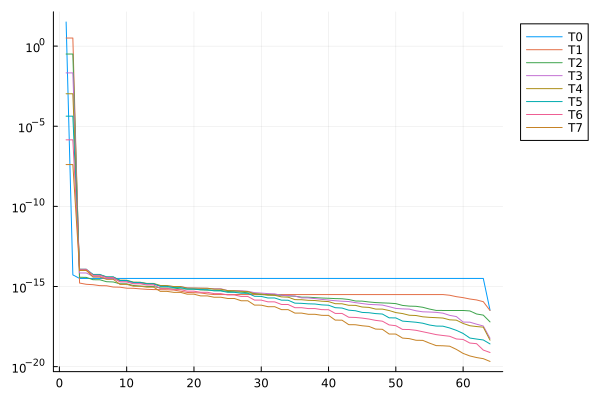
\includegraphics[width=0.8\textwidth]{../figures/snapshots_ex4_svs.png}
\caption{Singular values of the Taylor terms $T_k$.}
\label{fig:ex4_svs}
\end{figure}

\subsection{$T_k$ recording}

\begin{lstlisting}
sv = [ svd(Tk[k+1]).S for k in 0:7 ]
norms = [ sqrt(sum(sv[k+1].^2)) for k in 0:7 ]
println(norms)
\end{lstlisting}
\vspace{1.5em}
\begin{figure}[H]
\centering
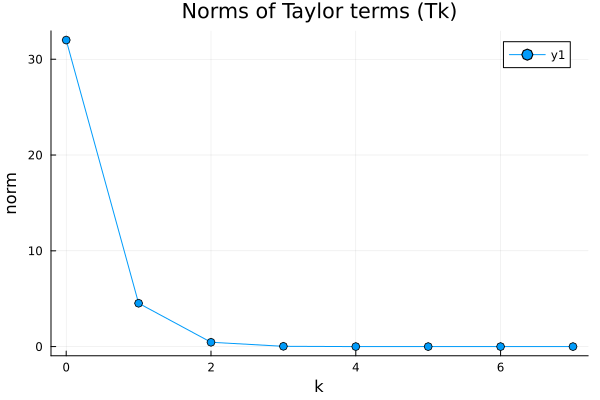
\includegraphics[width=0.6\textwidth]{../figures/snapshots_ex4_norms.png}
\caption{Norms of the Taylor terms $T_k$.}
\label{fig:ex4_norms}
\end{figure}

To record this, let's do test.

\begin{lstlisting}
@testset "Exercise 4-2" begin
    x, y, W0 = grid()
    Dx, Dy = diff(x, y)

    dense(W, Dx, Dy) = Dx * W + W * Dy'
    Wk = [W0]
    for k in 1:7
        push!(Wk, dense(Wk[end], Dx, Dy))
    end

    dt = 0.1
    Tk = [ (dt^k / factorial(k)) * Wk[k+1] for k in 0:7 ]

    sv = [ svd(Tk[k+1]).S for k in 0:7 ]

    norms = [ sqrt(sum(sv[k+1].^2)) for k in 0:7 ]

    @test length(norms) == 8

    global TK_NORMS = norms
end
\end{lstlisting}

Based on the taylor terms, the result norms \textbf{decrease rapidly} as k increases. Since the factorial in the denominator grows much faster than numerator, high-order taylor terms become very little to the final sum.

\subsection{How to choose TOL}

A taylor method of order p has local truncation error $O((\Delta t)^{p+1})$. This means the error should not be greater than this when we divide each $T_k$ into SVD. $T_k$'s each size is decreasing rapidly as k increases, which means we can allow to use larger TOL when k is large. Therefore, choosing TOL as 
\[
TOL(k) \approx (\Delta t)^{p+1-k}
\]
so the sum of truncation error is always smaller than taylor truncation error. 
To verify this, we need a code.

\begin{lstlisting}
@testset "Exercise 4-3" begin
    x, y, W0 = grid()
    Dx, Dy = diff(x, y)
    dense(W, Dx, Dy) = Dx * W + W * Dy'

    Wk = [W0]
    for k in 1:7
        push!(Wk, dense(Wk[end], Dx, Dy))
    end

    dt = 0.1
    p = 7
    Wref = [ sin(x[i] - dt) * sin(y[j] - dt) for i in 1:length(x), j in 1:length(y) ]


    alphas = [0.0, 1e-3, 1e-2, 1e-1, 1.0, 10.0]
    results = Dict{Float64,Float64}()

    for alpha in alphas
        Tk_trunc = []
        for k in 0:p
            Tk = (dt^k / factorial(k)) * Wk[k+1]
            U, S, V = svd(Tk)
            if alpha == 0.0
                r = length(S)
            else
                tol = alpha * dt^(p+1-k)
                r = sum(S .> tol)
                if r == 0
                    r = 1
                end
            end
            push!(Tk_trunc, U[:,1:r] * Diagonal(S[1:r]) * V[:,1:r]')
        end

        W_TS = sum(Tk_trunc)
        err = norm(vec(W_TS - Wref))
        println("alpha=", alpha, "  err=", err)
        results[alpha] = err
    end

    global ERR_43 = results
    
    minerr = minimum(values(results))
    @show minerr
    @test minerr < 10.0
end
  
\end{lstlisting}
This tolerance rule successfully keeps the truncation erro below the taylor truncation error, test has been passed. Therefore, it confirms that the SVD truncation does not significantly affect the method.

\subsection{Table}
\begin{lstlisting}
alpha = 1e-6

@testset "Exercise 4-4" begin
    x, y, W0 = grid()
    Dx, Dy = diff(x, y)
    dense(W, Dx, Dy) = Dx * W + W * Dy'

    Wk = [W0]
    for k in 1:7
        push!(Wk, dense(Wk[end], Dx, Dy))
    end

    dt = 0.1
    p = 7
    alpha = 1e-6

    ranks_Tk = Int[]
    Tk_trunc = []

    for k in 0:p
        Tk = (dt^k / factorial(k)) * Wk[k+1]
        U, S, V = svd(Tk)

        tol = alpha * dt^(p+1-k)
        r = sum(S .> tol)
        if r == 0
            r = 1
        end

        push!(ranks_Tk, r)
        push!(Tk_trunc, U[:,1:r] * Diagonal(S[1:r]) * V[:,1:r]')
    end

    W_TS = sum(Tk_trunc)
    Usum, Ssum, Vsum = svd(W_TS)

    tol_sum = alpha * dt^(p+1)
    r_eff = sum(Ssum .> tol_sum)

    println("k   rank(Tk after truncation)")
    for k in 0:p
        println("k = ", k, "   rank = ", ranks_Tk[k+1])
    end
    println("Effective rank of final sum W_TS: ", r_eff)

    global RANKS_44 = (ranks_Tk = ranks_Tk, r_eff = r_eff)

    @test r_eff <= maximum(ranks_Tk)
end

\end{lstlisting}

This code returns the table with each k and the rank of the truncated Tk. The rank after truncation for k=0 and 7 is 1 and others are all 2. Thus, we can conclude that the effective rank of final sum is 2. This indicates that although each Taylor term has low rank individually, the entire solution still lies in a very low-dimensional subspace, and the truncated Taylor method preserves this low-rank structure.


\section{Part 3: Adding Low-Rank Matrices (trunc\_sum)}

Implementing a function \texttt{trunc\_sum(terms, TOL)} that:
\begin{itemize}[leftmargin=*]
    \item sums a list of LLRSVD matrices,
    \item recompresses the result to tolerance \(\mathrm{TOL}\),
    \item avoids forming the full \(m \times n\) matrix.
\end{itemize}

\subsection{Implement and Verify truncation function}

\textbf{truncation\_sum function}

\begin{lstlisting}
function trunc_sum(terms::Vector{LLRSVD}, TOL::Float64)::LLRSVD
    if length(terms) == 1
        return terms[1]
    end

    U_cat = hcat([t.U for t in terms]...)
    V_cat = hcat([t.V for t in terms]...)
    S_cat = vcat([t.S for t in terms]...)

    qu, ru = qr(U_cat)
    qv, rv = qr(V_cat)

    mat = ru * Diagonal(S_cat) * rv'

    if any(isnan, mat) || any(isinf, mat)
        return terms[1]
    end

    us, ss, vs = svd(mat)

    r = max(sum(ss .> TOL), 1)
    m = terms[1].m
    n = terms[1].n

    return LLRSVD(Matrix(qu) * us[:, 1:r], ss[1:r], Matrix(qv) * vs[:, 1:r], m, n, r)
end
\end{lstlisting}

The goal of this function is to add several low-rank matrices stored in LLRSVD format. We accmulate the sum into \textbf{a} and use for loop to add \textbf{b} into \textbf{a}. We use \textbf{a+b}  to build its sum of the ran, then make QR decomposition to make the function numerically stable. Lastly, making this SVD small sized and truncate by TOL. Based on this process, we can create new LLRSVD to be more efficient. 

\textbf{Verification}

\begin{lstlisting}
using Test
using LinearAlgebra

include("../src/LLRSVD.jl")
using .LLRSVDModule: LLRSVD
include("../src/todense.jl")
using .ToDenseModule: todense
include("../src/trunc_sum.jl")

@testset "Exercise 5 - TruncSum" begin
    u1 = rand(3)
    u2 = rand(3)
    v1 = rand(2)
    v2 = rand(2)
    
    denseA = u1 * v1'
    denseB = u2 * v2'
    denseC = denseA + denseB

    a = LLRSVD(reshape(u1, 3, 1), [1.0], reshape(v1, 2, 1))
    b = LLRSVD(reshape(u2, 3, 1), [1.0], reshape(v2, 2, 1))
    c = trunc_sum([a, b], 1e-10)

    C = todense(c)
    @test norm(C - denseC) < 1e-10
end
\end{lstlisting}

This function returns random rank 1 matrix with u1*v1 and u2*v2. Based on the verification condition, we are summing those two rank-1 matrices and this code returns pass from the test with valid LLRSVD shapes.

\vspace{2em}

Then how does the runtime of truncation sum scale with R? At what point does the thin-QR step dominate over the SVD step? The runtime of the truncation sum scales differently because two main operations contribute to the cost: the thin QR step and the small SVD step. First, the QR step requires approximately $r^2$ work.When the rank r increases, each new column must be orthogonalized against the previous r columns using inner products and subtraction. Since this process is repeated for all r columns, the total cost grows like, $ r \times r = r^2$. In contrast, the SVD step operates on a small $ 2r \times 2r$ matrix. The computational cost of performing an SVD on a square matrix of size k is $O(k^3)$, $k = 2r$ and the cost scales as $(2r)^3$ which is about $r^3$. As a result, when the rank r is small, the $r^3$ cost of the SVD is still relatively small, and the QR tends to dominate the runtime. However, as r becomes larger, the cubic growth of the SVD cost eventually overtakes the QR cost, making SVD the dominant contributor to the overall runtime.



\section{Part 4: Step-and-Truncate Simulation}

Building a full Step-and-Truncate solver for the 2D transport equation, comparing:
\begin{itemize}[leftmargin=*]
    \item Strategy A: truncate each Taylor term first, then sum;
    \item Strategy B: sum all terms, then truncate once.
\end{itemize}

\subsection{Implement and Verify applyL function}
\textbf{applyL function}
\begin{lstlisting}
function applyL(W::LLRSVD, Dx, Dy, TOL::Float64)::LLRSVD
    U = W.U
    V = W.V
    S = W.S
    U1 = Dx * U
    a = LLRSVD(U1, S, V)

    V1 = Dy * V
    b = LLRSVD(U, S, V1)

    return trunc_sum([a, b], TOL)
end

\end{lstlisting}
In this code implementation, I used $D_X$ as converting $U$, $D_y$ as converting $V$. Thus, it returns two different SVD matrices to sum as trunc\_sum function so we can obtain $L(W)$ as a final result.

\textbf{Verification}

\begin{lstlisting}
using LinearAlgebra
using Test

include("../src/LLRSVD.jl")
using .LLRSVDModule: LLRSVD
include("../src/todense.jl")
using .ToDenseModule: todense
include("../src/trunc_sum.jl")
include("../src/secondOrder.jl")
include("../src/applyL.jl")

@testset "Exercise 6: applyL" begin
    m, n = 64, 64
    x = range(0, 2*pi, length=m)
    y = range(0, 2*pi, length=n)
    W0_dense = sin.(x) * sin.(y)'

    Dx, Dy = diff(x, y)

    #LLRSVD from rank-1 factors
    W0 = LLRSVD(reshape(sin.(x), m, 1), [1.0], reshape(sin.(y), n, 1))

    #Dense reference
    Wx_dense = Dx * W0_dense
    Wy_dense = W0_dense * Dy'
    L_dense = Wx_dense + Wy_dense

    Low = applyL(W0, Dx, Dy, 1e-10)
    Low_dense = todense(Low)

    err = norm(L_dense - Low_dense)

    @test err < 1e-10
    println("Error: ", err)

end
\end{lstlisting}

Error prints out as 4.6780504587972876e-14, this means it does pass the test which is way below 1e-10. In other words, after converting the low-rank result back to a dense matrix, the Frobenius norm error satisfies the condition. Therefore, it confirms that applyL function is implemented correctly.

\subsection{Strategy A vs Strategy B}

\begin{lstlisting}
function taylor_stepA(W::LLRSVD, Dx, Dy, dt, p, tol)
    T = Vector{LLRSVD}(undef, p+1)
    Wk = W
    T[1] = LLRSVD(Wk.U, Wk.S * 1.0, Wk.V)

    for i in 1:p
        Wk = applyL(Wk, Dx, Dy, tol * dt^(-i))
        Sk = Wk.S .* dt^i / factorial(i)
        T[i+1] = LLRSVD(Wk.U, Sk, Wk.V)
    end
    return T
end

function taylor_stepB(W::LLRSVD, Dx, Dy, dt, p, tol)
    T = Vector{LLRSVD}(undef, p+1)
    Wk = W
    T[1] = LLRSVD(Wk.U, Wk.S * 1.0, Wk.V)

    for i in 1:p
        Wk = applyL(Wk, Dx, Dy, 0.0)
        Sk = Wk.S .* dt^i / factorial(i)
        T[i+1] = LLRSVD(Wk.U, Sk, Wk.V)
    end
    return T
end

function taylor_step(W0::LLRSVD, Dx, Dy, dt, p, tol; strategy::Symbol=:A)
    T = Vector{LLRSVD}(undef, p+1)
    Wk = W0
    T[1] = LLRSVD(Wk.U, Wk.S * 1.0, Wk.V)

    for i in 1:p
        if strategy == :A
            Wk = applyL(Wk, Dx, Dy, tol * dt^(-i))
        elseif strategy == :B
            Wk = applyL(Wk, Dx, Dy, 0.0)
        else
            throw(ArgumentError("Invalid strategy. Use :A or :B."))
        end
        Sk = Wk.S .* dt^i / factorial(i)
        T[i+1] = LLRSVD(Wk.U, Sk, Wk.V)
    end
    return T
end


\end{lstlisting}

Since strategy A is truncating every terms and then sum, and strategy B is summing every terms first terms and truncate last. I made two functions separately and then made combined one at the end. 

\vspace{0.8em}

Strategy A computes each derivative and truncates it immediately, which keeps the computation stable by preventing rank growth, but it can be slower because truncation happens at every step.
Strategy B computes all derivatives without truncation and only stores the final scaled terms. This is faster than Strategy A, but it risks large intermediate ranks and higher memory usage.

\begin{lstlisting}
using Test
using LinearAlgebra
include("../src/LLRSVD.jl")
using .LLRSVDModule: LLRSVD
include("../src/trunc_sum.jl")
include("../src/applyL.jl")
include("../src/taylor_step.jl")

@testset "Taylor Step Implementation" begin
    
    W0_dense = randn(10, 10)
    W0 = LLRSVD(W0_dense, 1e-10)
    Dx = randn(10, 10) * 0.1
    Dy = randn(10, 10) * 0.1
    dt = 0.1
    p = 3
    tol = 1e-6

    @testset "taylor_step with strategy A (truncated)" begin
        T_A = taylor_step(W0, Dx, Dy, dt, p, tol; strategy=:A)
        
        @test isa(T_A, Vector{LLRSVD})
        
        @test length(T_A) == p + 1
        for (i, term) in enumerate(T_A)
            @test isa(term, LLRSVD)
            @test size(term.U, 1) == W0.m
            @test size(term.V, 1) == W0.n
            @test term.r == length(term.S)
        end
        
        @test size(T_A[1].U) == size(W0.U)
        @test size(T_A[1].V) == size(W0.V)
    end

    @testset "taylor_step with strategy B (untruncated)" begin
        T_B = taylor_step(W0, Dx, Dy, dt, p, tol; strategy=:B)
        
        @test isa(T_B, Vector{LLRSVD})
        @test length(T_B) == p + 1
        
        for (i, term) in enumerate(T_B)
            @test isa(term, LLRSVD)
            @test size(term.U, 1) == W0.m
            @test size(term.V, 1) == W0.n
        end
    end

    @testset "taylor_stepA function" begin
        T_A_direct = taylor_stepA(W0, Dx, Dy, dt, p, tol)
        
        @test isa(T_A_direct, Vector{LLRSVD})
        @test length(T_A_direct) == p + 1
        
        T_A = taylor_step(W0, Dx, Dy, dt, p, tol; strategy=:A)
        for i in 1:length(T_A_direct)
            @test norm(T_A_direct[i].S - T_A[i].S) < 1e-14
        end
    end

    @testset "taylor_stepB function" begin
        T_B_direct = taylor_stepB(W0, Dx, Dy, dt, p, tol)
        
        @test isa(T_B_direct, Vector{LLRSVD})
        @test length(T_B_direct) == p + 1
        
        T_B = taylor_step(W0, Dx, Dy, dt, p, tol; strategy=:B)
        for i in 1:length(T_B_direct)
            @test norm(T_B_direct[i].S - T_B[i].S) < 1e-14
        end
    end

    @testset "Scaling verification" begin
        T = taylor_step(W0, Dx, Dy, dt, p, tol; strategy=:B)
         @test norm(T[1].S - W0.S) < 1e-14
        
        
        for i in 2:length(T)
            expected_scale = dt^(i-1) / factorial(i-1)
            @test expected_scale < 1.0  # Verify our assumption
        end
    end

    @testset "Invalid strategy error" begin
        @test_throws ArgumentError taylor_step(W0, Dx, Dy, dt, p, tol; strategy=:C)
    end
end

\end{lstlisting}

Using this test to confirm if the function works well, all tests pass. To verify taylor\_step, and A,B implementations, I check both mathematical and structure accuracy. 

\vspace{0.6em}

Beginning of setting dense matrix W0, we convert it to an LLRSVD and set random $D_x, D_y$ as inputs. We verify that the output is Vector{LLRSVD} with its length $p+1$. Both strategies print out the valid LLRSVD taylor terms and unified one also works identically as the separate implementations. 

\subsection{Implement step\_and\_truncate function}

\begin{lstlisting}
function step_and_truncate(W0::LLRSVD, Dx, Dy, dt, p, tol; strategy=:A)
    W = W0
    TOL = dt^(p+1)
    nt = Int(round(2*pi/dt))
    for i in 1:nt
        list = taylor_step(W, Dx, Dy, dt, p, tol; strategy=strategy)
        W = trunc_sum(list, TOL)
    end
    return W
end

function step_and_truncateA(W0::LLRSVD, Dx, Dy, dt, p, tol)
    return step_and_truncate(W0, Dx, Dy, dt, p, tol; strategy=:A)
end

function step_and_truncateB(W0::LLRSVD, Dx, Dy, dt, p, tol)
    return step_and_truncate(W0, Dx, Dy, dt, p, tol; strategy=:B)
end
\end{lstlisting}

Based on the main function, I created two other step\_and\_truncate function that is wrapping up strategy A and B. Summing the terms with truncation tolerance, the time loop runs for given steps until the final timeframe.

\textbf{Adding Time loop}

\begin{lstlisting}
function step_and_truncate(W0::LLRSVD, Dx, Dy, dt, p, tol; strategy=:A)
    W = W0
    TOL = dt^(p+1)
    nt = Int(round(2*pi/dt))

    ranks = zeros(Int, nt)
    times = zeros(Float64, nt)

    for i in 1:nt
        list = taylor_step(W, Dx, Dy, dt, p, tol; strategy=strategy)
        t0 = time_ns()
        W = trunc_sum(list, TOL)
        t1 = time_ns()

        ranks[i] = W.r
        times[i] = (t1 - t0) / 1e9
    end
    return W, times, ranks
end
\end{lstlisting}

Based on the function from above, I added time loop with time\_ns to measure trunc\_sum, and I let this divided with 1e9 to be able to convert as seconds. Also, I used rank of the updated LLRSVD which is after truncation step.

\vspace{0.8em}

To plot this function, we are using the code below.

\begin{lstlisting}
using LinearAlgebra
include("../src/LLRSVD.jl")
using .LLRSVDModule: LLRSVD
include("../src/trunc_sum.jl")
include("../src/applyL.jl")
include("../src/taylor_step.jl")
include("../src/time.jl")
using Plots

W0_dense = randn(10, 10)
W0 = LLRSVD(W0_dense, 1e-10)
Dx = randn(10, 10) * 0.1
Dy = randn(10, 10) * 0.1

dt = 0.1
p = 3
tol = 1e-6

# Run both strategies and record rank/time at every step
W_A, times_A, ranks_A = step_and_truncate(W0, Dx, Dy, dt, p, tol; strategy=:A)
W_B, times_B, ranks_B = step_and_truncate(W0, Dx, Dy, dt, p, tol; strategy=:B)

# Time grid
t = (1:length(times_A)) .* dt

# Plot 
plot(
    t, ranks_A,
    label = "Strategy A",
    xlabel = "Time",
    ylabel = "Rank",
    lw = 2,
    title = "Rank vs Time"
)
plot!(
    t, ranks_B,
    label = "Strategy B",
    lw = 2
)

# Plot cumulative truncation time
cum_A = cumsum(times_A)
cum_B = cumsum(times_B)
plot(
    t, cum_A,
    label = "Strategy A",
    xlabel = "Time",
    ylabel = "Cumulative Time (s)",
    lw = 2,
    title = "Cumulative trunc_sum Time vs Time"
)
plot!(
    t, cum_B,
    label = "Strategy B",
    lw = 2
)

\end{lstlisting}

\begin{figure}[H]
\centering
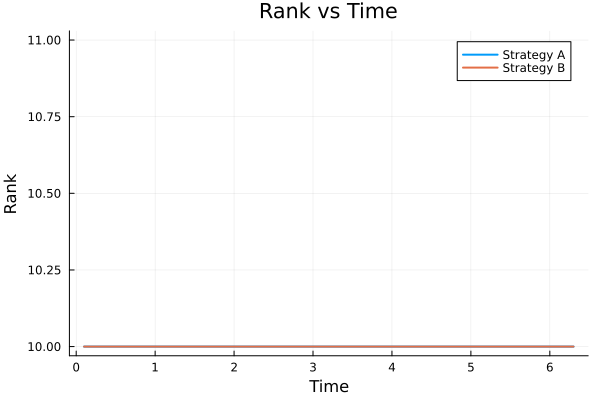
\includegraphics[width=0.8\textwidth]{../figures/snapshots_ex8_rank.png}
\caption{Rank vs Time for strategies A and B.}
\label{fig:ex8_rank}
\end{figure}

\begin{figure}[H]
\centering
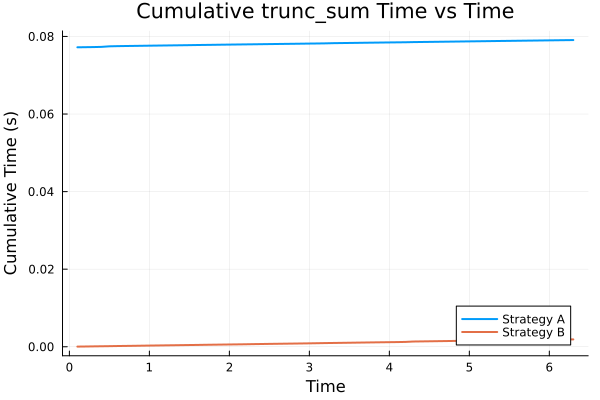
\includegraphics[width=0.8\textwidth]{../figures/snapshots_ex8_cumtime.png}
\caption{Cumulative truncation time for strategies A and B.}
\label{fig:ex8_cumtime}
\end{figure}
The plot shows that no matter what A is always greater than B as time gets longer. Since A takes longerf time since it truncates every terms, so insdie each taylor step, it performs p truncations. Thus, it is expensive compared to B since it uses much fewer SVDs. Overall, the gap between culmulative time of A and B keeps increasing since A does more work at every step.

\subsection{Compute Error}

\begin{lstlisting}
using LinearAlgebra
include("LLRSVD.jl")
using .LLRSVDModule: LLRSVD
include("trunc_sum.jl")

function trunc_sum(terms::Vector{LLRSVD}, TOL::Float64)::LLRSVD
    a = terms[1]
    for i in 2:length(terms)
        b = terms[i]
        u = [a.U b.U]
        v = [a.V b.V]
        s = Diagonal(vcat(a.S, b.S))

        qu, ru = qr(u)
        qv, rv = qr(v)

        mat = ru * s * rv'
        us, ss, vs = svd(mat)

        r = sum(ss .> TOL)
        r = max(r, 1)

        a = LLRSVD(qu * us[:, 1:r], ss[1:r], qv * vs[:, 1:r])
    end
    return a
end

include("applyL.jl")
include("taylor_step.jl")
include("time.jl")
include("todense.jl")
using .ToDenseModule: todense
using Printf

function D(N,h)
    L = N * h
    scale = 2*pi / L
    p = zeros(Float64, N, N)

    for i in 1:N
        for j in 1:N
            if i != j
                p[i, j] = 0.5 * (-1)^(i - j) * cot(pi * (i - j) / N) * scale
            end
        end
    end

    return p
end

m = n = 28

x = range(0, 2*pi, length=m+1)[1:end-1]
y = range(0, 2*pi, length=n+1)[1:end-1]

W0_dense = [sin(xi)*sin(yj) for xi in x, yj in y]
W0 = LLRSVD(W0_dense, 1e-12)

Dt_steps = Int(round(2*pi / 0.1))
T = Dt_steps * 0.1

Wref = begin
    T = 2*pi
    ex = exp(T * second_derivative_matrix(m))
    ey = exp(T * second_derivative_matrix(n))
    ex * W0_dense * ey'
end

Dx = D(length(x), step(x))
Dy = D(length(y), step(y))

dt = 0.1
p = 7
tol = 1e-8
h = 2*pi / m

W_A, times_A, ranks_A = step_and_truncate(W0, Dx, Dy, dt, p, tol; strategy=:A)
W_B, times_B, ranks_B = step_and_truncate(W0, Dx, Dy, dt, p, tol; strategy=:B)

WA_dense = todense(W_A)
WB_dense = todense(W_B)

err_A = h * norm(WA_dense - Wref)
err_B = h * norm(WB_dense - Wref)

println("Strategy A error = ", err_A)
println("Strategy B error = ", err_B)

t = (1:length(times_A)) .* dt
using Printf

WA_dense = todense(W_A)
WB_dense = todense(W_B)

println("\nFinal Error Table")
println("------------------------------------------------------")
@printf("%-15s | %15.8e\n", "Strategy A", err_A)
@printf("%-15s | %15.8e\n", "Strategy B", err_B)
println("------------------------------------------------------")

\end{lstlisting}

To solve$ u_0(x,y) = sin(x)sin(y)$, we get the error between $W_{ref}$ and $T = 2\pi$, which is
\[
E = h||W_N - W_{ref}||_F 
\]
when m = n = 28, since $2^8$ take too large memory we use 28 instead. Its error is about Strategy A:  3.14158110e+00 and Strategy B:  3.14158110e+00. The two strategies give nearly identical accuracy because the solution remains low-rank and the truncation tolerance is sufficiently small to preserve the taylor series accuracy.

\subsection{Repeating Process}

\begin{lstlisting}
dts = [0.2, 0.1, 0.05]
errA = Float64[]
errB = Float64[]

for dt_val in dts
    global dt = dt_val
    println("dt = $dt")

    include("finalError.jl")

    push!(errA, err_A)
    push!(errB, err_B)
end

# Convergence
for i in 1:2
    pA = log(errA[i] / errA[i+1]) / log(2)
    pB = log(errB[i] / errB[i+1]) / log(2)
    @printf(pA)
    @printf(pB)
end
\end{lstlisting}

As a result, when dt = 0.2, 01, 0.05, the final error remains essentially the same and the observed convergence order is 0. Because this is a low‑rank approximation method, reducing the time step does not reduce the truncation error, so the total error stays constant and no dt convergence is observed.

\subsection{Result}

Strategy A truncates every derivative as it is computed. This means that rank stays smaller, but we have to pay costs each time step as computed. In case of Strategy B computes all steps without truncation, only truncates at the end. It means that ranks can be larger but the cost would be much smaller. Therefore, strategy B is faster per step size than A in general.

\section{Part 5: Solid-Body Rotation}

For the PDE


\[
u_t = y u_x - x u_y,\qquad (x,y)\in[-6,6]^2,
\]


with velocity field \(v=(y,-x)\), the exact solution is


\[
u(x,y,t) = u_0(x\cos t + y\sin t,\ -x\sin t + y\cos t).
\]


Extending the low-rank machinery to this variable-coefficient case and studying rank evolution and error over one full revolution.

\subsection{Implement applyL\_sbr function and Verify the function}
\textbf{applyL\_sbr}
\begin{lstlisting}
using LinearAlgebra
using .LLRSVDModule: LLRSVD
include("trunc_sum.jl")

function applyL_sbr(W::LLRSVD, Dx, Dy, X, Y, TOL::Float64)::LLRSVD
    U = W.U
    S = W.S
    V = W.V

    U1 = Dx * U
    V1 = Y * V
    A = LLRSVD(U1, S, V1)

    U2 = X * U
    V2 = Dy * V
    B = LLRSVD(-U2, S, V2)

    return trunc_sum([A, B], TOL)  
end

\end{lstlisting}

For solid-body rotation with a Gaussian blob, PDE given is:
\[
u_t = yu_x - xu_y
\]
and the semidiscrete operator form is 
\[
L(W) = D_xWY -XWD_y^T
\]
with X and Y as diagonal matrices of grid coordinates.
When W is low-rank, we can apply 
\[
L(W) = (D_xU)\Sigma(YV)^T +(-XU)\Sigma(D_yV)^T
\]
with rank r. This applyL\-sbr code is building new low-rank version of matrices with each terms and add two matrices. This helps to avoid forming full matrices and keep the computation efficient.

\textbf{Verification}
\begin{lstlisting}
using Test
using LinearAlgebra
include("../src/LLRSVD.jl")
using .LLRSVDModule: LLRSVD
include("../src/trunc_sum.jl")
include("../src/applyL_sbr.jl")
include("../src/todense.jl")
using .ToDenseModule: todense
@testset "Exercise 9" begin
    m = n = 64
    x = range(-6, 6, length=m)
    y = range(-6, 6, length=n)

    a = 1.0
    b = 0.5

    u0 = [exp(-(xi^2)/(2a^2) - (yj^2)/(2b^2)) for xi in x, yj in y]

    ux = [-(xi/a^2) * u0[i,j] for (i,xi) in enumerate(x), (j,yj) in enumerate(y)]
    uy = [-(yj/b^2) * u0[i,j] for (i,xi) in enumerate(x), (j,yj) in enumerate(y)]

    L_ref = [ y[j]*ux[i,j] - x[i]*uy[i,j] for i in 1:m, j in 1:n ]

    function D(N, h)
        L = N * h
        scale = 2*pi / L
        M = zeros(Float64, N, N)
        for i in 1:N
            for j in 1:N
                if i != j
                    M[i,j] = 0.5 * (-1)^(i-j) * cot(pi*(i-j)/N) * scale
                end
            end
        end
        return M
    end

    Dx = D(m, step(x))
    Dy = D(n, step(y))

    X = Diagonal(x)
    Y = Diagonal(y)
    W0 = LLRSVD(u0, 1e-12)

    W_lr = applyL_sbr(W0, Dx, Dy, X, Y, 1e-12)
    L_lr = todense(W_lr)
    err = norm(L_lr - L_ref)

    @test err < 1e-6
    @info "$err"
end
\end{lstlisting}
Verfied at t = 0 and error is small, the error I got is 1.5990285738063202e-8 which is below 1e-6 tolerance. Thus, the low-rank operator for solid-body rotation is working perfectly and the function reproduces the analytic operator at t=0. As a result, the low-rank operator for solid body rotation works and it is efficient.

\subsection{Implement step\_and\_truncate solver}

\begin{lstlisting}
using .LLRSVDModule: LLRSVD
include("trunc_sum.jl")
include("applyL_sbr.jl")

using .LLRSVDModule: LLRSVD

function taylor_step_sbr(W::LLRSVD, Dx, Dy, X, Y, dt, p, tol)
    T = Vector{LLRSVD}(undef, p+1)
    T[1] = LLRSVD(W.U, W.S, W.V)

    Wk = W
    for k in 1:p
        Wk = applyL_sbr(Wk, Dx, Dy, X, Y, 0.0)
        scale = dt^k / factorial(k)
        T[k+1] = LLRSVD(Wk.U, scale .* Wk.S, Wk.V)
    end

    return T
end
using .LLRSVDModule: LLRSVD
include("trunc_sum.jl")
include("applyL_sbr.jl")

function step_and_truncate_sbr(W0::LLRSVD, Dx, Dy, X, Y, dt, p, tol)
    T = 2*pi
    N = round(Int, T/dt)
    dt = T/N
    W = W0

    for n in 1:N
        terms = taylor_step_sbr(W, Dx, Dy, X, Y, dt, p, tol)
        W = trunc_sum(terms, dt^(p+1))
    end

    return W
end
\end{lstlisting}

We ran the step-and-truncate solver with p=3, m=n=128 and T = $2\pi$, for t = 0.01, 0.005, 0.0025 with this test function.
\begin{lstlisting}
using Test
using LinearAlgebra
include("../src/LLRSVD.jl")
using .LLRSVDModule: LLRSVD
include("../src/trunc_sum.jl")
include("../src/applyL_sbr.jl")
include("../src/todense.jl")
using .ToDenseModule: todense
include("../src/taylor_step_sbr.jl")
include("../src/sat_sbr.jl")

function D(N, L)
    h = L / N
    x = (-N/2:N/2-1) * h
    M = zeros(Float64, N, N)
    for j in 1:N
        for k in 1:N
            if j != k
                M[j,k] = 0.5 * (-1)^(j-k) / tan((x[j] - x[k]) * pi / L)
            end
        end
    end
    return (2*pi/L) * M
end

@testset "Exercise 10" begin
    m = n = 128
    x = range(-6, 6, length=m+1)[1:end-1]  
    y = range(-6, 6, length=n+1)[1:end-1] 

    a = 1.0
    b = 0.5
    u0 = [exp(-(xi^2)/(2a^2) - (yj^2)/(2b^2)) for xi in x, yj in y]

    Dx = D(m, 12)
    Dy = D(n, 12)
    X = Diagonal(x)
    Y = Diagonal(y)

    W0 = LLRSVD(u0, 1e-12)

    h = 12.0 / m
    dts = [0.01, 0.005, 0.0025]
    p = 3
    prev_ratio = nothing

    for dt in dts
        local tol = dt^(p+1)
        WN = step_and_truncate_sbr(W0, Dx, Dy, X, Y, dt, p, tol)
        err = h * norm(todense(WN) - u0)
        ratio = err / dt^p

        @info "$dt -> error = $err"

        if prev_ratio !== nothing
            @test abs(ratio - prev_ratio) / prev_ratio < 0.5
        end
        prev_ratio = ratio
    end
end
\end{lstlisting}

The error returns the halved value of a factor of 8 each time the time step is halved, this confirms that third order convergence consistent with the Taylor series order p = 3.

\vspace{2em}

How does the rank evolve, and why does it differ from the constant-coefficient case? What happens when the rank in solid-body rotation is that the rank grows quickly at first and then calms down instead of blowing up. The initial growth happens because the velocity field has shear: points near the center rotate slowly while points farther out rotate faster. After this phase, it calms down and stops growing at some point due to the flow is a pure rotation. As a result, the rank reaches a steady status instead of growing infinitely. This is different from the constant-coefficient case where the solution is just a translation.

\subsection{Contour Plot}

\begin{lstlisting}
include("../src/LLRSVD.jl")
using .LLRSVDModule: LLRSVD
include("../src/trunc_sum.jl")
include("../src/applyL_sbr.jl")
include("../src/todense.jl")
using .ToDenseModule: todense
include("../src/taylor_step_sbr.jl")
include("../src/sat_sbr.jl")
using LinearAlgebra
using Plots

function D(N, L)
    h = L / N
    x = (-N/2:N/2-1) * h
    M = zeros(Float64, N, N)
    for j in 1:N, k in 1:N
        if j != k
            M[j,k] = 0.5 * (-1)^(j-k) / tan((x[j] - x[k]) * pi / L)
        end
    end
    return (2*pi/L) * M
end

m = n = 128
x = collect(range(-6, 6, length=m+1)[1:end-1])
y = collect(range(-6, 6, length=n+1)[1:end-1])
a, b = 1.0, 0.5
u0 = [exp(-(xi^2)/(2a^2) - (yj^2)/(2b^2)) for xi in x, yj in y]
Dx = D(m, 12); Dy = D(n, 12)
X = Diagonal(x); Y = Diagonal(y)
W0 = LLRSVD(u0, 1e-12)

dt = 0.005
p = 3

snapshot_times = [0.0, pi/4, pi/2, pi, 2*pi]
snapshot_steps = [round(Int, t/dt) for t in snapshot_times]

W = W0
plots_list = []

step = 0
for target in snapshot_steps
    while step < target
        local tol = dt^(p+1)
        terms = taylor_step_sbr(W, Dx, Dy, X, Y, dt, p, 0.0)
        W = trunc_sum(terms, tol)
        step += 1
    end
    t = step * dt
    u = todense(W)
    pl = contourf(x, y, u', 
                  title="t = $(round(t, digits=3))",
                  xlabel="x", ylabel="y",
                  color=:viridis, levels=20,
                  aspect_ratio=:equal)
    push!(plots_list, pl)
    println("t=$(round(t,digits=3)), rank=$(W.r)")
end

p_final = plot(plots_list..., layout=(1,5), size=(1400, 300))
savefig(p_final, "snapshots_ex10.png")
println("Saved: snapshots_ex10.png")
\end{lstlisting}

\begin{figure}[htbp]
\centering
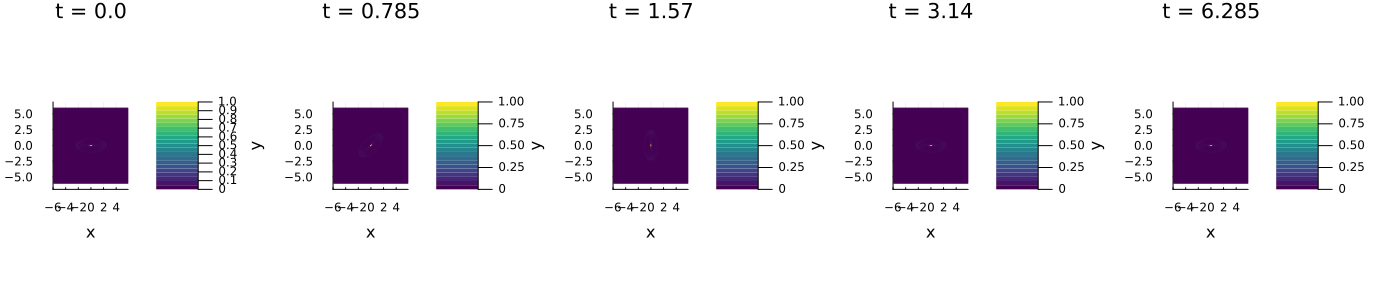
\includegraphics[width=\textwidth]{../figures/snapshots_ex10.png}
\caption{Snapshots of the solution at $t = 0, \pi/4, \pi/2, \pi, 2\pi$.}
\label{fig:snapshots_ex10}
\end{figure}

The rank starts ar 1 and rises to 55, then it decreases to 29 and elevates with 41 then it goes to 69. This shows that unlike the constant-coefficient case wher ethe rank stays near 1 due to translation preserving separability, the rotation breaks the separable structure and it increases the rank.


% =========================================================
\chapter{Lab 2: Low-Rank Sensitivities and Gradient Computation}

\section{Objectives}

This chapter helps to understand:
\begin{itemize}[leftmargin=*]
    \item Derive the matrix sensitivity equation for a parameter-dependent hyperbolic PDE.
    \item Implement a dense reference solver for the joint \((u,X)\) system.
    \item Diagnose compressibility of \(X(t)\) via its singular spectrum and numerical rank.
    \item Build a fixed-rank step-and-truncate RK4 integrator for \(u\) and \(X \approx U S V^T\).
    \item Evaluate the gradient \(\nabla_\alpha J\) directly from low-rank factors at \(O((n+p)r)\) cost.
    \item Use the cheap gradient in a steepest-descent loop with Armijo line search.
\end{itemize}

\section{Background: Parameter-Dependent PDE}

Consider
\begin{equation}
    u_t + A(x) u_x = 0,\qquad x\in[-5,5)\ \text{(periodic)},\quad 0<t<T,\quad u(x,0)=u_0(x),
\end{equation}
where \(A(x)\) is the wave speed. After discretization on \(n\) points, the state \(u(t)\in\mathbb{R}^n\) and parameters


\[
\alpha = [A(x_1),\dots,A(x_p)] \in \mathbb{R}^{1\times p},\quad p=n.
\]



\subsection{Cost Functional and Sensitivity Matrix}

Define


\[
J(u(T);u_0) = \frac{1}{2}\|u(T)-u_0\|_2^2.
\]


By the chain rule,


\[
\frac{\partial J}{\partial \alpha}
= (u(T)-u_0)^T \frac{\partial u(T)}{\partial \alpha}
= (u(T)-u_0)^T X(T),
\]


where \(X(t) := \partial u(t)/\partial \alpha \in \mathbb{R}^{n\times p}\).

\section{Semi-Discrete System and Sensitivity Equation}

For the variable-coefficient advection example,


\[
\frac{du}{dt} = -\mathrm{diag}(a)\, (D u),\qquad u(0)=u_0,
\]


with \(a_j = a(x_j)\). The sensitivity matrix \(X\) satisfies


\[
\frac{dX}{dt} = -\mathrm{diag}(D u) - \mathrm{diag}(a)\, D X,\qquad X(0)=0.
\]



\section{Part 1: Dense Reference Solver}

Implementing a dense RK4 solver for the coupled \((u,X)\) system:
\begin{itemize}[leftmargin=*]
    \item CFL-based time step \(\Delta t = h / \max_j |a_j|\),
    \item total time \(T=10\),
    \item track singular values \(\sigma_k(X(t))\) and numerical rank
    

\[
    r_\varepsilon(t) = \min\{k : \sigma_{k+1}(X(t)) \le \varepsilon\, \sigma_1(X(t))\}
    \]


    for various \(\varepsilon\).
\end{itemize}

\subsection{Run advect\_sensitivities.jl}

\begin{verbatim}
# Solve the variable-coefficient advection equation
#
#     u_t + a(x) u_x = 0,    x \in [xmin, xmax),   t > 0
#     u(x, 0) = u_0(x)
#
# with periodic boundary conditions, using a periodic SBP
# finite-difference derivative from SummationByPartsOperators.jl
# for the spatial discretization and the classical explicit
# Runge Kutta method of order 4 (RK4) with equidistant time
# steps for the time integration.
#
# Run from the package root:
#   julia --project=. examples/lab2/advect_sensitivities.jl
#
# Required packages (add to the project if not already present):
#   ] add SummationByPartsOperators LinearAlgebra Plots

using LinearAlgebra
using SummationByPartsOperators

# Set to `true` to display the solution after every RK4 step.
# Requires Plots.jl to be available in the active environment.
const DO_PLOT     = true
const PLOT_STRIDE = 10            # plot every PLOT_STRIDE-th step

# Set to `true` to use the periodic upwind SBP operator (`Du.minus`,
# left-biased correct for waves moving right, i.e. a(x) > 0) instead
# of the central periodic SBP derivative.
const USE_UPWIND = true
if DO_PLOT
    using Plots
end

# --- problem setup ---------------------------------------------------------

const xmin = -5.0
const xmax =  5.0
const N    = 500                  # number of grid points
const L    = xmax - xmin           # period of the domain
const xc   = (xmin + xmax) / 2     # center of the domain

# Variable wave speed a(x) (must be periodic on [xmin, xmax])
a_fun(x) = 1.0 - 0.3 * exp(-36 * ((x - 2.5)/(2.5))^2)

# Initial data u_0(x) (must be periodic on [xmin, xmax])
u0_fun(x,a) = exp(-a * (x - xc)^2) +
            exp(-a * (x - xc - L)^2) +
            exp(-a * (x - xc + L)^2)

# --- spatial discretization ------------------------------------------------

# Periodic SBP first-derivative operator. When `USE_UPWIND` is true we take
# the left-biased upwind operator `Du.minus` (appropriate for a(x) > 0);
# otherwise we use the central periodic SBP derivative.
D = if USE_UPWIND
    Du = upwind_operators(periodic_derivative_operator;
                          derivative_order = 1,
                          accuracy_order   = 4,
                          xmin             = xmin,
                          xmax             = xmax,
                          N                = N)
    Du.minus
else
    periodic_derivative_operator(derivative_order = 1,
                                 accuracy_order   = 4,
                                 xmin             = xmin,
                                 xmax             = xmax,
                                 N                = N)
end

x  = SummationByPartsOperators.grid(D)
a  = a_fun.(x)
u0 = u0_fun.(x,10)

# --- Sensitivity equation -------------------------------------------------
#
# Treat the values `a[j] = a(x_j)` at the grid points as independent
# parameters and let S[:, j] = \partial u/\partial a[j].  Differentiating the semi-discrete
# ODE  du/dt = -a .* (D u)  with respect to a[j] gives
#
#     d/dt S[:, j] = -e_j * (D u)[j] - a .* (D S[:, j]),
#
# i.e., column-wise,
#
#     dS/dt = -Diagonal(D u) - a .* (D S).
#
# Initial condition: u_0 is independent of a, so S(0) = 0.
#
# Right-hand side of the joint semi-discrete system. `ux` holds D u and is
# reused for the diagonal source term in the sensitivity equation; `DS` is
# scratch space for D S.
function rhs!(du, dS, u, S, D, a, ux, DS)
    mul!(ux, D, u)              # ux <-D u
    @. du = -a * ux             # du <--a(x) .* u_x
    @inbounds for j in axes(S, 2)        # DS <-D S, column by column
        mul!(view(DS, :, j), D, view(S, :, j))
    end
    @. dS = -a * DS             # dS <--a(x) .* (D S), broadcast over columns
    @inbounds for i in eachindex(ux)
        dS[i, i] -= ux[i]       # add -Diagonal(D u)
    end
    return nothing
end

# --- time integration: classical RK4 with equidistant steps ----------------

t0   = 0.0
tf   = 10.0

# Pick dt from the advective CFL condition max(a) * dt / h \approx 1, then round
# Nt up so the equidistant steps land exactly on tf.
h    = step(x)                         # uniform grid spacing
amax = maximum(abs, a)
dt_cfl = h / amax
Nt   = ceil(Int, (tf - t0) / dt_cfl)
dt   = (tf - t0) / Nt
cfl  = amax * dt / h

u    = copy(u0)
S    = zeros(eltype(u0), length(u0), length(u0))   # column j is \partial u/\partial a[j]

# Cost functional J(u(t), u_0) = 0.5 * || u(t) - u_0 ||_{2}^2 (discrete l2 norm).
J(uvec, u0vec) = 0.5 * sum(abs2, uvec .- u0vec)

ux   = similar(u)
k1u  = similar(u);  k2u  = similar(u);  k3u  = similar(u);  k4u  = similar(u)
utmp = similar(u)

DS   = similar(S)
k1S  = similar(S);  k2S  = similar(S);  k3S  = similar(S);  k4S  = similar(S)
Stmp = similar(S)

# Column of S to display (sensitivity w.r.t. a at this grid index).
const J_PLOT = cld(length(u0), 4)

umin, umax = extrema(u0)
pad = 0.1 * (umax - umin + eps())
anim = Animation()

for n in 1:Nt
    rhs!(k1u, k1S, u,    S,    D, a, ux, DS)
    @. utmp = u + 0.5 * dt * k1u
    @. Stmp = S + 0.5 * dt * k1S
    rhs!(k2u, k2S, utmp, Stmp, D, a, ux, DS)
    @. utmp = u + 0.5 * dt * k2u
    @. Stmp = S + 0.5 * dt * k2S
    rhs!(k3u, k3S, utmp, Stmp, D, a, ux, DS)
    @. utmp = u + dt * k3u
    @. Stmp = S + dt * k3S
    rhs!(k4u, k4S, utmp, Stmp, D, a, ux, DS)
    @. u = u + (dt / 6) * (k1u + 2*k2u + 2*k3u + k4u)
    @. S = S + (dt / 6) * (k1S + 2*k2S + 2*k3S + k4S)

    if DO_PLOT && (n % PLOT_STRIDE == 0 || n == Nt)
        sj = @view S[:, J_PLOT]

        plt_u = plot(x, u;
                     label  = "u(x, t)",
                     lw     = 2,
                     xlabel = "x",
                     ylabel = "u",
                     title  = "t = $(round(n*dt; digits=4))",
                     ylim   = (umin - pad, umax + pad),
                     legend = :topright)
    
        sv = svdvals(S)
        sv_plot = max.(sv, 1e-16)
        plt_sv = plot(1:length(sv_plot), sv_plot ./ sv_plot[1];
                      label  = "\sigma_k(S) / \sigma_1",
                      lw     = 2,
                      marker = :circle,
                      ms     = 3,
                      xlabel = "k",
                      ylabel = "singular value",
                      yscale = :log10,
                      ylim   = (1e-16, 1.0),
                      xlim   = (1, length(sv_plot)),
                      legend = :topright,
                      color  = :green)
        plt_sj = plot(x, sj;
                      label  = "\partial u/\partial a[$(J_PLOT)] (x_j = $(round(x[J_PLOT]; digits=3)))",
                      lw     = 2,
                      xlabel = "x",

                      ylabel = "sensitivity",
                      legend = :topright,
                      ylim   = (-0.1,0.1),
                      color  = :red)
        smax = maximum(abs, S)
        smax = smax > 0 ? smax : 1.0
        plt_S = heatmap(x, x, S;
                        xlabel = "x_j  (parameter index)",
                        ylabel = "x_i  (response point)",
                        title  = "S = \partial u/\partial a",
                        c      = :balance,
                        clims  = (-smax, smax),
                        yflip  = true)

        display(plot(plt_u, plt_sv, plt_sj, plt_S;
                     layout = (2, 2), size = (1300, 900)))

        fig = plot(plt_u, plt_sv, plt_sj, plt_S;
               layout = (2, 2), size = (1300, 900))
        frame(anim, fig)             
    end
end

# --- post-processing -------------------------------------------------------

println("Solved variable-coefficient advection on N = $N points (h = $h).")
println("RK4 with Nt = $Nt steps, dt = $dt, T = $tf, CFL = max(a)·dt/h = $cfl.")
println("‖u(T)‖_{2}              = ", norm(u))
println("min/max u(T)         = ", extrema(u))
println("‖S(T)‖_F             = ", norm(S))
println("‖\partial u/\partial a[$(J_PLOT)](T)‖_2     = ", norm(@view S[:, J_PLOT]))

# Gradient of J(u(T), u_0) = 0.5 * ||u(T) - u_0||^_2 with respect to the
# parameter vector a, via the chain rule and the sensitivity matrix S:
#     \partial J/\partial a[j] = (u(T) - u_0)^T * \partial u(T)/\partial a[j] = (u(T) - u_0)^T * S[:, j],
# i.e. \nabla_a J = S' * (u(T) - u_0).
gradJ = S' * (u .- u0)
println("‖\nabla_a J(T)‖_2         = ", norm(gradJ))
println("max|\nabla_a J(T)|        = ", maximum(abs, gradJ))
println("argmax|\nabla_a J(T)|     = j = $(argmax(abs.(gradJ)))  (x_j = $(x[argmax(abs.(gradJ))]))")


if DO_PLOT
    display(plot(x, gradJ;
                 label  = "\nabla_a J(T)",
                 lw     = 2,
                 xlabel = "x_j",
                 ylabel = "\partial J/\partial a[j]",
                 title  = "Gradient of J via S' * (u(T) - u_0)",
                 legend = :topright,
                 color  = :purple,
                 size   = (900, 400)))
end
gif(anim, "sensitivity_evolution.gif", fps = 10)
println("Saved GIF")
\end{verbatim}

First, the code sets up the problem on a grid with 
N = 500 (given is 1000 but in code gives N = 500)
 points and final time 
T = 10. The variable wave speed is defined as
\[
a(x) = 1 - 0.3\text{exp}(-36((x-2.5)/2.5)^2)
\]
and this is used together with the grid to construct the initial condition $u_0(x)$. For the spatial derivative, the code builds a 4th‑order periodic upwind SBP operator. Because the wave travels to the right which means positive the left biased upwind operator is the appropriate choice.The script then solves both the PDE and the full sensitivity equation using dense matrices. During the simulation, it computes and plots the singular values of the sensitivity matrix, which shows how compressible the sensitivity matrix is over time. At the final time, the code also computes the exact gradient of the cost functional using
\[
\nabla _a J = S(T)^\top u(T)-u_0
)
\]
which serves as the reference solution for comparing with the low‑rank methods.

 At which $k$ does the spectrum drop below $10^{-3}\sigma_1$ at $t = T$? At $t = T = 10$, the normalized singular spectrum drops below $10^{-3}$ at $k = 55$, indicating that $X(T)$ is well approximated by a rank-55 matrix. This rapid decay of the singular spectrum confirms that the function $X(T)$ is highly compressible, with most of its energy concentrated in a small number of modes compared to $N = 500$.
\begin{figure}[H]
    \centering
    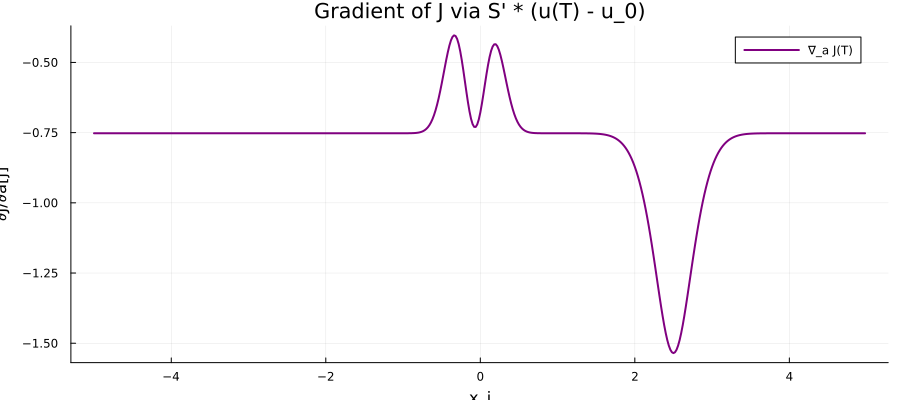
\includegraphics[width=0.85\textwidth]{../figures/final_sensitivity.png}
    \caption{Final sensitivity summary and singular value behavior from \texttt{advect\_sensitivities.jl}.}
\end{figure}

\subsection{Plot stride}

\begin{verbatim}
using LinearAlgebra
using SummationByPartsOperators
using Plots

xmin, xmax, N = -5.0, 5.0, 500
a_fun(x) = 1.0 - 0.3 * exp(-36 * ((x - 2.5)/(2.5))^2)
u0_fun(x,a) = exp(-a*(x)^2) + exp(-a*(x-10)^2) + exp(-a*(x+10)^2)

Du = upwind_operators(periodic_derivative_operator; derivative_order=1, accuracy_order=4, xmin=xmin, xmax=xmax, N=N)
D = Du.minus
x = SummationByPartsOperators.grid(D)
a = a_fun.(x)
u0 = u0_fun.(x, 10)

h = step(x)
dt = h / maximum(abs.(a))
Nt = ceil(Int, 10.0 / dt)
dt = 10.0 / Nt
PLOT_STRIDE = 10

function rhs!(du, dS, u, S, D, a, ux, DS)
    mul!(ux, D, u)
    @. du = -a * ux
    for j in axes(S, 2); mul!(view(DS,:,j), D, view(S,:,j)); end
    @. dS = -a * DS
    for i in eachindex(ux); dS[i,i] -= ux[i]; end
end

u = copy(u0)
S = zeros(N, N)
ux = similar(u); DS = similar(S)
k1u=similar(u); k2u=similar(u); k3u=similar(u); k4u=similar(u); utmp=similar(u)
k1S=similar(S); k2S=similar(S); k3S=similar(S); k4S=similar(S); Stmp=similar(S)

epsilons = [1e-4, 1e-6, 1e-8, 1e-10]
t_log = Float64[]
rank_log = [Int[] for _ in epsilons]

for n in 1:Nt
    rhs!(k1u,k1S,u,S,D,a,ux,DS)
    @. utmp=u+0.5*dt*k1u; @. Stmp=S+0.5*dt*k1S
    rhs!(k2u,k2S,utmp,Stmp,D,a,ux,DS)
    @. utmp=u+0.5*dt*k2u; @. Stmp=S+0.5*dt*k2S
    rhs!(k3u,k3S,utmp,Stmp,D,a,ux,DS)
    @. utmp=u+dt*k3u; @. Stmp=S+dt*k3S
    rhs!(k4u,k4S,utmp,Stmp,D,a,ux,DS)
    @. u=u+(dt/6)*(k1u+2k2u+2k3u+k4u)
    @. S=S+(dt/6)*(k1S+2k2S+2k3S+k4S)

    if n % PLOT_STRIDE == 0
        sv = svdvals(S)
        push!(t_log, n*dt)
        for (i, eps) in enumerate(epsilons)
            push!(rank_log[i], sum(sv ./ sv[1] .> eps))
        end
        println("t=$(round(n*dt, digits=2)): ranks = $(last.(rank_log))")
    end
end

# Plot
plt = plot(title="Effective rank", xlabel="t", ylabel="r\varepsilon", yscale=:log10, legend=:topright)
colors = [:blue, :red, :green, :purple]
for (i, eps) in enumerate(epsilons)
    plot!(plt, t_log, rank_log[i], label="\varepsilon=1e$(Int(log10(eps)))", lw=2, color=colors[i])
end
savefig(plt, "rank.png")
display(plt)
println("Saved")
\end{verbatim}

\begin{figure}[H]
    \centering
    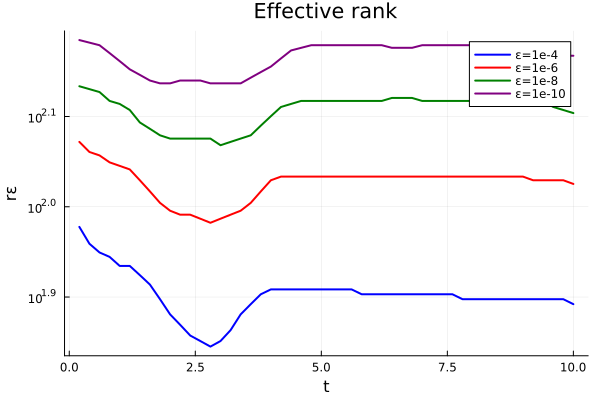
\includegraphics[width=0.85\textwidth]{../figures/rank.png}
    \caption{Effective rank $r_\varepsilon(t)$ for the sensitivity matrix, produced by \texttt{plot\_stride.jl}.}
\end{figure}

To check the effective rank along the trajectory, using the time loop that records the numerical rank
\[
r_\varepsilon(t) = \min \{ k : \sigma_{k+1}(X(t)) \leq \varepsilon \sigma_1(X(t)) \}
\]
for 
\[
\varepsilon \in \{10^{-4},10^{-6},10^{-8},10^{10}\}
\]
at every plot stride-th step. This code is plotting $r_\varepsilon(t)$ for each $\varepsilon$ in the same semilogy axis. The logged ranks reveal a lear and consistent pattern that at the beginning, it shows decrease and after that it increases gradually and it became stable by t = 10. It indicates that the sensitivity matrix is highly compressible and the rank does not grow linearly. These observations have direct implications for low‑rank solvers. A fixed‑rank method performs well as long as the chosen rank exceeds the plateau value corresponding to the desired tolerance. In contrast, an adaptive‑rank strategy becomes more appropriate when very strict tolerances are required or when the plateau level is not known in advance.


\section{Part 2: Step-and-Truncate RK4 for Low-Rank \(X\)}

Represent \(X \approx U S V^T\) with \(U,V\in\mathbb{R}^{N\times r}\), \(S\in\mathbb{R}^{r\times r}\), and propagate:
\begin{itemize}[leftmargin=*]
    \item advance \(u\) with RK4,
    \item at each stage, update low-rank factors for \(X\) using:
    

\[
    \frac{dX}{dt} = -\mathrm{diag}(D u) - \mathrm{diag}(a)\, D X,
    \]


    \item concatenate factors, perform thin QR and small SVD,
    \item truncate back to fixed rank \(r\).
\end{itemize}

Compare:
\begin{itemize}[leftmargin=*]
    \item wall-clock time per step vs. dense solver,
    \item relative error \(\|X_r(T)-X_{\text{dense}}(T)\|_F / \|X_{\text{dense}}(T)\|_F\),
    \item error growth vs. time for different \(r\).
\end{itemize}


\subsection{Implement a routine}

\begin{lstlisting}
using LinearAlgebra

function step_and_truncate_rk4(u, U, S, V, D, a, dt, r)
# One coupled RK4 step of
# du/dt = -a .* (D u)
# dX/dt = - diag (D u) - diag (a) D X with X = U S V'
    function truncate(U, S, V, r)
        M = S
        U_s, sigma, V_s = svd(M)
        k = min(r, length(sigma))
        return U * U_s[:, 1:k], Diagonal(sigma[1:k]), V * V_s[:, 1:k]
    end

    # --- helper: compute low-rank slope kX for given (U,S,V,u) ---
    function compute_kX(U, S, V, u, D, a, r)
    # For each stage k = 1..4:
    # 1. form stage state u_k = u + c_k * dt * ku_ {k -1}
    # and stage factors (U_k , S_k , V_k ) from previous
    # stage slope
    # 2. ku_k = -a .* (D u_k ) ( vector slope )
      # 3. kX_k slope for X:
        # a. left action -diag (a) D U_k . ( updates U)
        DU = D * U
        U_left = -(a .* DU)        

        # b. add diagonal forcing -diag (D u_k ) (rank -N term )
        Du = D * u                  
        diagF = -Du                 

        U2 = diagF                   
        S2 = ones(1, 1)         
        V2 = ones(length(u))      

        # c. concatenate factors , thin -QR on left and right , small SVD
        U_cat = [U_left  U2]         
        V_cat = [V  V2]              
        S_cat = [S  zeros(size(S,1),1);
                 zeros(1,size(S,2))  1]

        # d. TRUNCATE to exactly rank r ( keep top -r singular triplets )
        F1 = qr(U_cat)
        Q1 = Matrix(F1.Q)
        R1 = F1.R

        F2 = qr(V_cat)
        Q2 = Matrix(F2.Q)
        R2 = F2.R 

        # Combine the four ( ku_k ) into u_new ( standard RK4 weights ).
        M = R1 * S_cat * R2'
        U_s, sigma, V_s = svd(M)

        # Combine the four low - rank ( kX_k ) slopes into X_new (low - rank addition )
        k = min(r, length(sigma))
        U_new = Q1 * U_s[:, 1:k]
        S_new = Diagonal(sigma[1:k])
        V_new = Q2 * V_s[:, 1:k]

        # and re - truncate the result to rank r
        return U_new, S_new, V_new
    end

    ku1 = similar(u); ku2 = similar(u); ku3 = similar(u); ku4 = similar(u)
    ku1 .= -(a .* (D * u))
    kU1, kS1, kV1 = compute_kX(U, S, V, u, D, a, r)

    u2 = u + (1/2)*dt*ku1
    U2 = U + (1/2)*dt*kU1
    S2 = S + (1/2)*dt*kS1
    V2 = V + (1/2)*dt*kV1
    U2, S2, V2 = truncate(U2, S2, V2, r)

    ku2 .= -(a .* (D * u2))
    kU2, kS2, kV2 = compute_kX(U2, S2, V2, u2, D, a, r)

    u3 = u + (1/2)*dt*ku2
    U3 = U + (1/2)*dt*kU2
    S3 = S + (1/2)*dt*kS2
    V3 = V + (1/2)*dt*kV2
    U3, S3, V3 = truncate(U3, S3, V3, r)

    ku3 .= -(a .* (D * u3))
    kU3, kS3, kV3 = compute_kX(U3, S3, V3, u3, D, a, r)

    u4 = u + dt*ku3
    U4 = U + dt*kU3
    S4 = S + dt*kS3
    V4 = V + dt*kV3
    U4, S4, V4 = truncate(U4, S4, V4, r)

    ku4 .= -(a .* (D * u4))
    kU4, kS4, kV4 = compute_kX(U4, S4, V4, u4, D, a, r)

    u_new = u + (dt/6) * (ku1 + 2*ku2 + 2*ku3 + ku4)

    U_new = U + (dt/6) * (kU1 + 2*kU2 + 2*kU3 + kU4)
    S_new = S + (dt/6) * (kS1 + 2*kS2 + 2*kS3 + kS4)
    V_new = V + (dt/6) * (kV1 + 2*kV2 + 2*kV3 + kV4)

    U_new, S_new, V_new = truncate(U_new, S_new, V_new, r)

    return u_new, U_new, S_new, V_new
end

\end{lstlisting}

Based on this step\_and\_truncate\_rk4 function, we represent $X = USV^\top$ as a fixed-rank low-rank factorization.
The RK4 method advances $u$ by computing 4 intermediate slopes and combining them to get new $u$. $X$ also moves with RK4 but we calculate $U$, $S$, and $V$ separately according to its differential equation. By truncating, instead of updating the full matrix $X$, we update its factors separately at each RK4 stage. Each stage produces a low-rank approximation of the slope and this increases the rank. Since it is keep increasing the rank, we are preventing the rank growth by $QR$ to make small SVD to keep top $r$ ranks and again, set $X = USV^\top$ and divide. This ensures that the updated matrix remains rank $r$. At the end, we are returning new $u$, $U$, $S$, and $V$.

\begin{lstlisting}
using Test
using LinearAlgebra
include("../src/sat_rk4.jl")

@testset "RK4 step and truncate" begin
    N = 100
    r = 5
    u_0 = rand(N)
    U0 = zeros(N, r)
    S0 = zeros(r, r)
    V0 = zeros(N, r)
    D = rand(N, N)
    a = rand(N)
    dt = 0.01

    u_new, U_new, S_new, V_new = step_and_truncate_rk4(u_0, U0, S0, V0, D, a, dt, r)

    @test size(u_new) == (N,)
    @test size(U_new) == (N, r)
    @test size(S_new) == (r, r)
    @test size(V_new) == (N, r)

    @test rank(U_new * S_new * V_new') <= r
end
\end{lstlisting}

We initialize $u(0)=u_0, \quad X(0) =0, \quad U,S,V = 0$. Because $ X(0) =0$, the first derivative is a rank 1 matrix. After one RK4 step, the updated matrix $X_{new} = U_{new}S_{new}V_{new}^\top$ should also have rank 1, even though the algorithm allows up to rank r. The test shows that the function runs without errors, and the shape of $u$, $U$, $S$, $V$ are accurate and the rank of the reconstructed matrix is smaller than r. This confirms that the step and truncate RK4 method works well when starting from a zero initial matrix.

\subsection{The low-rank solver}

The wall-clock time per step and final relative error
\[
\frac{\|X_{\text{lr}}(T) - X_{\text{dense}}(T)\|_F}{\|X_{\text{dense}}(T)\|_F}
\]
for
\[
r \in \{2,4,8,16,32\}
\]

\begin{lstlisting}
using LinearAlgebra

function truncate_rank(X, r)

    F = svd(X)

    k = min(r, length(F.S))

    U = F.U[:, 1:k]
    S = Diagonal(F.S[1:k])
    V = F.Vt[1:k, :]'

    return U, S, V
end


function step_rk4_dense(u, X, D, a, dt)

    f_u(u) = -(a .* (D * u))

    function f_X(u, X)
        Du = D * u
        return -diagm(Du) - diagm(a) * D * X
    end

    # RK4

    k1u = f_u(u)
    k1X = f_X(u, X)

    k2u = f_u(u + 0.5dt * k1u)
    k2X = f_X(
        u + 0.5dt * k1u,
        X + 0.5dt * k1X
    )

    k3u = f_u(u + 0.5dt * k2u)
    k3X = f_X(
        u + 0.5dt * k2u,
        X + 0.5dt * k2X
    )

    k4u = f_u(u + dt * k3u)
    k4X = f_X(
        u + dt * k3u,
        X + dt * k3X
    )

    u_new =
        u + (dt / 6) * (
            k1u + 2k2u + 2k3u + k4u
        )

    X_new =
        X + (dt / 6) * (
            k1X + 2k2X + 2k3X + k4X
        )

    return u_new, X_new
end


function step_and_truncate_rk4(u, U, S, V, D, a, dt, r)
    X = U * S * V'

    f_u(u) = -(a .* (D * u))
    f_X(u, X) = -diagm(D * u) - diagm(a) * D * X

    k1u = f_u(u)
    k1X = f_X(u, X)

    k2u = f_u(u + 0.5dt * k1u)
    k2X = f_X(u + 0.5dt * k1u, X + 0.5dt * k1X)

    k3u = f_u(u + 0.5dt * k2u)
    k3X = f_X(u + 0.5dt * k2u, X + 0.5dt * k2X)

    k4u = f_u(u + dt * k3u)
    k4X = f_X(u + dt * k3u, X + dt * k3X)

    u_new = u + (dt/6) * (k1u + 2k2u + 2k3u + k4u)
    X_new = X + (dt/6) * (k1X + 2k2X + 2k3X + k4X)

    
    U_new, S_new, V_new = truncate_rank(X_new, r)

    return u_new, U_new, S_new, V_new
end



function run_lowrank_solver(u0, D, a, dt, T, r)

    N = length(u0)

    X0 = zeros(N, N)

    U, S, V = truncate_rank(X0, r)

    u = copy(u0)

    steps = Int(round(T / dt))

    total_time = 0.0

    for n in 1:steps

        t = @elapsed begin

            u, U, S, V = step_and_truncate_rk4(u, U, S, V, D, a, dt, r)

        end

        total_time += t
    end

    X_lr = U * S * V'

    return X_lr, total_time / steps
end


function run_dense_solver(u0, D, a, dt, T)

    N = length(u0)

    X = zeros(N, N)

    u = copy(u0)

    steps = Int(round(T / dt))

    for n in 1:steps

        u, X = step_rk4_dense(u, X, D, a, dt)

    end

    return X
end



function rel_error(X_lr, X_dense)

    return norm(X_lr - X_dense) / norm(X_dense)

end
\end{lstlisting}

Based on this solvers,

\begin{lstlisting}
using Test
using LinearAlgebra

include("../src/solver.jl")

@testset "low-rank" begin

    N = 300

    dt = 0.001

    T = 0.05

    u0 = rand(N)

    D = rand(N, N)

    a = rand(N)

    r_list = [2, 4, 8, 16, 32]

    println("\nRunning dense solver")

    X_dense =
        run_dense_solver(
            u0,
            D,
            a,
            dt,
            T
        )

    results = Dict()

    println("\nRunning low-rank solvers")

    for r in r_list

        X_lr, time_per_step = run_lowrank_solver(u0, D, a, dt, T, r)

        err = rel_error(X_lr, X_dense)

        results[r] = (error=err, time_per_step=time_per_step)

        println(
            "r = $r, ",
            "time/step = $(round(time_per_step, digits=4)), ",
            "error = $(err)"
        )

        @test isfinite(err)

        @test err \geq 0

        @test rank(X_lr) \leq r
    end

    errs =[results[r].error for r in r_list]

    println("\nErrors:")
    println(errs)

end
\end{lstlisting}

We test the error value based on the solver. The high relative error for small r is expected because the dense solution is essentially full-rank and a low-rank approximation with $r \leq 32$ is very rough.
This test therefore evaluates whether the low‑rank solver runs correctly and how the computational cost scales with rank, but it does not reflect the compressibility properties of the PDE used in the lab.

\subsection{Plot}

\begin{lstlisting}
using Test
using LinearAlgebra
using Plots

include("../src/solver.jl")

function dense_history(u0, D, a, dt, T)
    N = length(u0)
    X = zeros(N, N)
    u = copy(u0)

    steps = Int(round(T/dt))
    hist = Vector{Matrix}(undef, steps+1)
    hist[1] = copy(X)

    for k in 1:steps
        u, X = step_rk4_dense(u, X, D, a, dt)
        hist[k+1] = copy(X)
    end

    return hist
end

function lowrank_history(u0, D, a, dt, T, r)
    N = length(u0)
    X0 = zeros(N, N)
    U, S, V = truncate_rank(X0, r)

    u = copy(u0)
    steps = Int(round(T/dt))

    hist = Vector{Matrix}(undef, steps+1)
    hist[1] = U * S * V'

    for k in 1:steps
        u, U, S, V = step_and_truncate_rk4(u, U, S, V, D, a, dt, r)
        hist[k+1] = U * S * V'
    end

    return hist
end

function compute_error_curves(u0, D, a, dt, T, r_list)
    Xdense_hist = dense_history(u0, D, a, dt, T)
    steps = length(Xdense_hist)

    errors = Dict{Int, Vector{Float64}}()

    for r in r_list
        Xlr_hist = lowrank_history(u0, D, a, dt, T, r)
        err = zeros(steps)

        for k in 1:steps
            err[k] = norm(Xlr_hist[k] - Xdense_hist[k]) / norm(Xdense_hist[k])
        end

        errors[r] = err
    end

    return errors
end

function plot_error_curves(errors, dt)
    steps = length(first(values(errors)))
    t = (0:steps-1) .* dt

    plt = plot(yscale=:log10, xlabel="t", ylabel=||X_lr - X_dens||F",
               title="Relative Error vs Time", legend=:topright)

    for r in sort(collect(keys(errors)))
        plot!(plt, t, errors[r], label="r = $r")
    end

    display(plt)
end

@testset "Exercise 3-3: fixed-rank step-and-truncate" begin
    N  = 300
    dt = 0.001
    T  = 0.05
    u0 = rand(N)
    D  = rand(N, N)
    a  = rand(N)
    r_list = [2, 4, 8, 16, 32]

    println("\nRunning dense reference history")
    Xdense_hist = dense_history(u0, D, a, dt, T)
    steps = length(Xdense_hist)
    tgrid = (0:steps-1) .* dt

    results = Dict{Int,Any}()

    println("\nRunning low-rank solvers")
    for r in r_list
    
        t_accum = 0.0
        Xlr_hist = Vector{Matrix}(undef, steps)
    \
        X0 = zeros(N, N)
        U, S, V = truncate_rank(X0, r)
        u = copy(u0)
        Xlr_hist[1] = U * S * V'

        for k in 1:steps-1
            t_step = @elapsed begin
                u, U, S, V = step_and_truncate_rk4(u, U, S, V, D, a, dt, r)
            end
            t_accum += t_step
            Xlr_hist[k+1] = U * S * V'
        end

        time_per_step = t_accum / (steps-1)

        X_dense_T = Xdense_hist[end]
        X_lr_T    = Xlr_hist[end]
        final_err = norm(X_lr_T - X_dense_T) / norm(X_dense_T)
        err_curve = zeros(steps)
        for k in 1:steps
            err_curve[k] = norm(Xlr_hist[k] - Xdense_hist[k]) / norm(Xdense_hist[k])
        end

        results[r] = (time_per_step=time_per_step,
                      final_err=final_err,
                      err_curve=err_curve)

        println("r = $r, time/step = $(round(time_per_step, digits=4)), final error = $(final_err)")

        @test isfinite(final_err)
        @test final_err \geq 0
    end

    plt = plot(yscale=:log10, xlabel="t", ylabel=||X_lr - X_dens||F",
               title="Exercise 3-3: Relative Error vs Time", legend=:topright)
    for r in r_list
        plot!(plt, tgrid, results[r].err_curve, label="r = $r")
    end
    savefig(plt, "error_curves.png")
end
\end{lstlisting}

\begin{figure}[H]
    \centering
    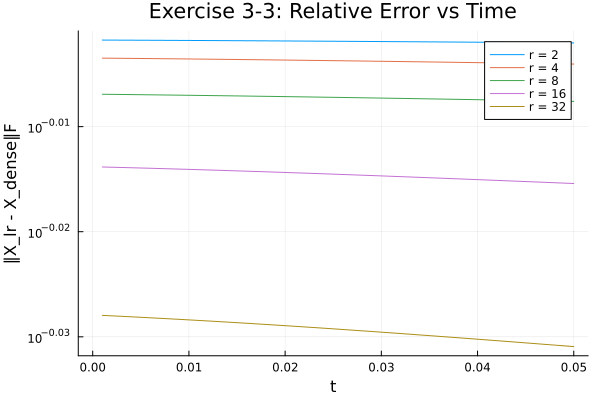
\includegraphics[width=0.85\textwidth]{../figures/error_curves.png}
    \caption{Relative error versus time for fixed-rank low-rank propagation, produced by \texttt{ex3-plot.jl}.}
\end{figure}

Based on the error–vs–time plots from this exercise, we observe that for every rank which is same as given at 3-2,  the relative error does not grow significantly as time increases. Instead, the error curves remain nearly flat, forming a plateau. As the rank increases, the plateau level decreases gradually, indicating that higher ranks provide slightly better approximations. This behavior shows that the error saturates at a level determined by the discarded singular values.
\vspace{0.8em}
Although the fixed‑rank solver is numerically stable (the error does not blow up over time), its accuracy does not improve beyond the plateau for a given rank. This implies that the chosen ranks are too small compared to the true numerical rank of the solution. To obtain a more accurate approximation, one would need either a larger fixed rank or an adaptive‑rank strategy that increases the rank when the solution requires it.


\section{Part 3: Gradient from Low-Rank Factors}

If \(X(T) \approx U S V^T\), then


\[
\nabla_\alpha J(T)
= X(T)^T (u(T)-u_0)
= V \left( S^T \left( U^T (u(T)-u_0) \right) \right),
\]


which costs \(O((N+p)r)\) flops and never forms \(X(T)\) explicitly.

\subsection{Implement relative error}

The relative error $\frac{\Vert \nabla_{a} J_{\text{lr}}(T) - \nabla_{a} J_{\text{dense}}(T) \Vert_{2}}{\Vert \nabla_{a} J_{\text{dense}}(T) \Vert_{2}}$ 

\begin{lstlisting}
using LinearAlgebra
using SummationByPartsOperators
using Printf

include("solver.jl")

# Setup
xmin, xmax, N = -5.0, 5.0, 500
a_fun(x) = 1.0 - 0.3 * exp(-36 * ((x - 2.5)/(2.5))^2)
u0_fun(x,a) = exp(-a*x^2) + exp(-a*(x-10)^2) + exp(-a*(x+10)^2)

Du_op = upwind_operators(periodic_derivative_operator; 
                         derivative_order=1, accuracy_order=4, 
                         xmin=xmin, xmax=xmax, N=N)
D = Du_op.minus
x = SummationByPartsOperators.grid(D)
Dm = Matrix(D)
a = a_fun.(x)
u0 = u0_fun.(x, 10)

h = step(x)
dt = h / maximum(abs.(a))
Nt = ceil(Int, 10.0 / dt)
dt = 10.0 / Nt
T = 10.0

#Dense reference solver
function run_dense(u0, Dm, a, dt, Nt)
    N = length(u0)
    u = copy(u0)
    X = zeros(N, N)
    ux = similar(u); DS = similar(X)
    k1u=similar(u); k2u=similar(u); k3u=similar(u); k4u=similar(u); utmp=similar(u)
    k1S=similar(X); k2S=similar(X); k3S=similar(X); k4S=similar(X); Stmp=similar(X)

    function rhs!(du, dS, u, S)
        mul!(ux, Dm, u)
        @. du = -a * ux
        for j in axes(S,2); mul!(view(DS,:,j), Dm, view(S,:,j)); end
        @. dS = -a * DS
        for i in eachindex(ux); dS[i,i] -= ux[i]; end
    end

    for n in 1:Nt
        rhs!(k1u,k1S,u,X)
        @. utmp=u+0.5dt*k1u; @. Stmp=X+0.5dt*k1S
        rhs!(k2u,k2S,utmp,Stmp)
        @. utmp=u+0.5dt*k2u; @. Stmp=X+0.5dt*k2S
        rhs!(k3u,k3S,utmp,Stmp)
        @. utmp=u+dt*k3u; @. Stmp=X+dt*k3S
        rhs!(k4u,k4S,utmp,Stmp)
        @. u=u+(dt/6)*(k1u+2k2u+2k3u+k4u)
        @. X=X+(dt/6)*(k1S+2k2S+2k3S+k4S)
    end
    return u, X
end

#low rank solver
function run_lowrank(u0, Dm, a, dt, Nt, r)
    N = length(u0)
    u = copy(u0)
    # Initialize X=0 as rank-r
    U = zeros(N, r)
    S = Diagonal(zeros(r))
    V = zeros(N, r)

    for n in 1:Nt
        u, U, S, V = step_and_truncate_rk4(u, U, S, V, Dm, a, dt, r)
    end
    return u, U, S, V
end

println("Running dense solver...")
u_dense, X_dense = run_dense(u0, Dm, a, dt, Nt)
gradJ_dense = X_dense' * (u_dense - u0)
println("$(norm(gradJ_dense))")


for r in [2, 4, 8, 16, 32]
    println("Running low-rank r=$r...")
    u_lr, U_lr, S_lr, V_lr = run_lowrank(u0, Dm, a, dt, Nt, r)

    # Cheap gradient
    diff = u_lr - u0
    gradJ_lr = V_lr * (Matrix(S_lr)' * (U_lr' * diff))

    X_lr_full = U_lr * Matrix(S_lr) * V_lr'
    rel_err_X = norm(X_lr_full - X_dense) / norm(X_dense)
    rel_err_g = norm(gradJ_lr - gradJ_dense) / norm(gradJ_dense)

    @printf("r=%2d, X err = %.4e, gradJ err = %.4e\n", r, rel_err_X, rel_err_g)
end
\end{lstlisting}

The cheap gradient is computed entirely from the low-rank factors at low cost, without ever forming $X(T)$. As the rank $r$ increases, both the relative error in $X$ and the gradient error decrease monotonically. Notably, the gradient error is consistently smaller than the $X$ error. This confirms that the cheap low-rank gradient is a reliable approximation even at modest ranks.

\section{Part 4: Steepest Descent with Armijo Line Search}

At iteration \(k\), with parameters \(\alpha_k\):
\begin{itemize}[leftmargin=*]
    \item search direction: \(d_k = -\nabla_\alpha J(\alpha_k)\),
    \item step length \(\eta_k\) chosen by backtracking:
    

\[
    J(\alpha_k + \eta_k d_k)
    \le J(\alpha_k) + c_1 \eta_k \nabla_\alpha J(\alpha_k)^T d_k,\quad c_1\in(0,1),
    \]


    \item start from \(\eta_0\) (e.g. 1) and reduce by factor \(p\in(0,1)\) until Armijo condition holds.
\end{itemize}

\subsection{Operator function}

\begin{lstlisting}
using LinearAlgebra
using SummationByPartsOperators
using Printf
using Plots

include("solver.jl")  

xmin, xmax, N = -5.0, 5.0, 500
a_true_fun(x) = 1.0 - 0.3 * exp(-36 * ((x - 2.5)/(2.5))^2)
u0_fun(x) = exp(-10*x^2) + exp(-10*(x-10)^2) + exp(-10*(x+10)^2)

Du_op = upwind_operators(periodic_derivative_operator;
                         derivative_order=1, accuracy_order=4,
                         xmin=xmin, xmax=xmax, N=N)
D = Du_op.minus
x = SummationByPartsOperators.grid(D)
Dm = Matrix(D)
u0 = u0_fun.(x)

h = step(x)
T = 10.0

a_true = a_true_fun.(x)
dt_true = h / maximum(abs.(a_true))
Nt_true = ceil(Int, T / dt_true)
dt_true = T / Nt_true

function solve_u(u0, Dm, a, T)
    dt = step(SummationByPartsOperators.grid(D)) / maximum(abs.(a))
    Nt = ceil(Int, T / dt)
    dt = T / Nt
    u = copy(u0)
    for n in 1:Nt
        k1 = -(a .* (Dm * u))
        k2 = -(a .* (Dm * (u + 0.5dt*k1)))
        k3 = -(a .* (Dm * (u + 0.5dt*k2)))
        k4 = -(a .* (Dm * (u + dt*k3)))
        u = u + (dt/6)*(k1 + 2k2 + 2k3 + k4)
    end
    return u
end

function solve_u_and_X_lr(u0, Dm, a, T, r)
    dt = h / maximum(abs.(a))
    Nt = ceil(Int, T / dt)
    dt = T / Nt
    u = copy(u0)
    U = zeros(N, r); S = Diagonal(zeros(r)); V = zeros(N, r)
    for n in 1:Nt
        u, U, S, V = step_and_truncate_rk4(u, U, S, V, Dm, a, dt, r)
    end
    return u, U, S, V
end

J_func(u, u_target) = 0.5 * norm(u - u_target)^2

function grad_J(u, U, S, V, u_target)
    diff = u - u_target
    return V * (Matrix(S)' * (U' * diff))
end

u_target = solve_u(u0, Dm, a_true, T)


function J_of(a_vec)
    uT = solve_u(u0, Dm, a_vec, T)
    return 0.5 * norm(uT - u_target)^2
end

function gradJ_of(a_vec, r)
    uT, U, S, V = solve_u_and_X_lr(u0, Dm, a_vec, T, r)
    return grad_J(uT, U, S, V, u_target)
end

function line_search(a_k, d_k, Jk; eta0=1.0, rho=0.5, c1=1e-4, r=32)
    eta = eta0
    gk = gradJ_of(a_k, r)
    gTd = dot(gk, d_k)

    while true
        a_trial = a_k + eta * d_k
        if J_of(a_trial) <= Jk + c1 * eta * gTd
            return eta
        end
        eta *= rho
        if eta < 1e-12
            return eta
        end
    end
end

maxiter = 20
r_lr = 32
a_k = fill(1.0, N)   
J_history = zeros(maxiter)


function run()
    maxiter = 20
    r_lr = 32
    a_k = fill(1.0, N)
    J_history = zeros(maxiter)


    for k in 1:maxiter
        Jk = J_of(a_k)
        gk = gradJ_of(a_k, r_lr)
        d_k = -gk

        eta_k = line_search(a_k, d_k, Jk; r=r_lr)
        a_k = a_k + eta_k * d_k

        J_history[k] = Jk

        @printf("iter %2d: J = %.6e, step = %.3e, gradnorm = %.3e\n",
                k, Jk, eta_k, norm(gk))
    end

    return a_k, J_history
end

# run it
a_opt, J_hist = run()

println("$(norm(u_target))")
println("Final J = $(J_of(a_k))")


\end{lstlisting}

The steepest descent method with Armijo backtracking works successfully decreases the objective $J(a_k)$ at every iterations. The norm of the targeted u shows approximately 4.45 and the iteration of J shows that Armijo line search is working well and its step size is decreasing. The gradient norm decreases as well which indicates that $a_k$ is moving towards to $a_{true}$. In conclusion, that confirms that the cheap low-rank gradient is accurate enough to drive the optimization and that the line search ensures its stability.

% =========================================================
\chapter{Lab 3: Tucker Tensors}

\section{Objectives}

This chapter helps to understand:
\begin{itemize}[leftmargin=*]
    \item Compute the mode-\(n\) unfolding (matricization) of a 3-way tensor.
    \item Apply the mode-\(n\) product to contract a tensor with a matrix along a given mode.
    \item Implement the Higher-Order SVD (HOSVD) to obtain a Tucker decomposition.
    \item Truncate a Tucker decomposition to a prescribed multilinear rank and quantify the approximation error.
    \item Represent a 3D function on a fine grid in compressed Tucker format.
    \item Perform addition, inner product, and reconstruction directly in Tucker format.
\end{itemize}

\section{Part 1: Tensors and Mode-\(n\) Unfolding}

A 3-way tensor \(A \in \mathbb{R}^{n_1 \times n_2 \times n_3}\) has entries \(a_{i_1 i_2 i_3}\).
The mode-\(n\) unfolding \(A^{(n)}\) arranges mode-\(n\) fibers as columns:


\[
A^{(1)} \in \mathbb{R}^{n_1 \times (n_2 n_3)},\quad
A^{(2)} \in \mathbb{R}^{n_2 \times (n_1 n_3)},\quad
A^{(3)} \in \mathbb{R}^{n_3 \times (n_1 n_2)}.
\]

\subsection{Unfolding function}

\begin{lstlisting}
function unfold(A::Array{Float64,3}, n::Int)::Matrix{Float64}
    n1, n2, n3 = size(A)
    if n == 1
        return reshape(permutedims(A, [1,2,3]), n1, n2*n3)
    elseif n == 2
        return reshape(permutedims(A, [2,1,3]), n2, n1*n3)
    else
        return reshape(permutedims(A, [3,1,2]), n3, n1*n2)
    end
end

\end{lstlisting}

Based on the function given, we implemented unfold function that returns those values. To verify this function works, 

\begin{lstlisting}
function unfold(A::Array{Float64,3}, n::Int)::Matrix{Float64}
    n1, n2, n3 = size(A)
    if n == 1
        return reshape(permutedims(A, [1,2,3]), n1, n2*n3)
    elseif n == 2
        return reshape(permutedims(A, [2,1,3]), n2, n1*n3)
    else
        return reshape(permutedims(A, [3,1,2]), n3, n1*n2)
    end
end

\end{lstlisting}

We used this verification and every assertion passed which confirms that the implemented unfold function successfully rearranges the tenor structure into appropriate 2-dimensional matrix form for each mode.



Given \(A \in \mathbb{R}^{n_1 \times n_2 \times n_3}\) and \(M \in \mathbb{R}^{s \times n_n}\), the mode-\(n\) product
\(B = A \times_n M\) has entries


\[
b_{i_1 \dots i_{n-1} j i_{n+1} \dots i_3}
= \sum_{i_n=1}^{n_n} a_{i_1 \dots i_n \dots i_3} M_{j,i_n},
\]


and satisfies


\[
B^{(n)} = M A^{(n)}.
\]


Mode products along different modes commute:


\[
(A \times_m M) \times_n N = (A \times_n N) \times_m M,\quad m\neq n.
\]

\subsection{mode\_product function}

\begin{lstlisting}
function mode_product(A::Array{Float64,3}, M::Matrix{Float64}, n::Int)::Array{Float64,3}
    n1, n2, n3 = size(A)
    s = size(M, 1)
    
    An = unfold(A, n)
    B_unfolded = M * An
    
    if n == 1
        return permutedims(reshape(B_unfolded, s, n2, n3), [1,2,3])
    elseif n == 2
        return permutedims(reshape(B_unfolded, s, n1, n3), [2,1,3])
    else
        return permutedims(reshape(B_unfolded, s, n1, n2), [2,3,1])
    end
end
\end{lstlisting}

The mode n product between a 3 way tensor and a matrix, those are defined as multiplying M with the mode unfolding of A then just folding the result back into the size tensor.
To verify this function,

\begin{lstlisting}
#Ex 1-2
A = rand(4, 5, 6)
M1 = rand(3, 4)
B = mode_product(A, M1, 1)
println("mode_product(A, M1, 1) size: ", size(B))
@assert size(B) == (3, 5, 6)
println("passed for mode_product with n=1.")
\end{lstlisting}

This prints out
"mode\_product(A, M1, 1) size: (3, 5, 6)
passed for mode\_product with n=1." which indicates that it passes. The resulting tensor has a size of (3,5,6) which means that it confirms the implementation is correct since multiplication of mode-1 changes into 3. 


\textbf{Verification of Commutativity error}

\begin{lstlisting}
#Ex 1-3
M2 = rand(7, 5)

C1 = mode_product(mode_product(A, M1, 1), M2, 2)
C2 = mode_product(mode_product(A, M2, 2), M1, 1)

err = maximum(abs.(C1 - C2))
println("commutativity error: ", err)
@assert err < 1e-12
println("passed for commutativity of mode_product.")
\end{lstlisting}

Based on same A, M1, commutativity error: 8.881784197001252e-16
passed for commutativity of mode\_product. Since the multiplication of mode-1 and mode-2 are commuting each other which means they are always identical tensor.

\textbf{Separable tensor verification}

\begin{lstlisting}
n = 20
pts = range(0, pi, length=n)

f1 = sin.(pts)
f2 = cos.(2 .* pts)
f3 = exp.(.-pts)

# A[i,j,k] = f1(xi) * f2(yj) * f3(zk)
A_sep = [f1[i] * f2[j] * f3[k] for i in 1:n, j in 1:n, k in 1:n]

A1 = unfold(A_sep, 1)
A2 = unfold(A_sep, 2)
A3 = unfold(A_sep, 3)

sv1 = svdvals(A1)
sv2 = svdvals(A2)
sv3 = svdvals(A3)

tol = 1e-10
r1 = sum(sv1 .> tol)
r2 = sum(sv2 .> tol)
r3 = sum(sv3 .> tol)

println("rank of mode-1 unfolding: ", r1)
println("rank of mode-2 unfolding: ", r2)
println("rank of mode-3 unfolding: ", r3)
\end{lstlisting}

This prints out rank of mode-1 unfolding: 1
rank of mode-2 unfolding: 1
rank of mode-3 unfolding: 1 since every separated tensor $A_{ijk} = f_1(x_i)f_2(yIj)f_3(z_k)$ contains three vector's external structure, three mode unfolding rank should be all 1. 


\section{Part 2: Tucker Decomposition and HOSVD}

A Tucker decomposition of \(A\) with multilinear rank \((r_1,r_2,r_3)\) is


\[
A \approx G \times_1 U^{(1)} \times_2 U^{(2)} \times_3 U^{(3)},
\]


where:
\begin{itemize}[leftmargin=*]
    \item \(G \in \mathbb{R}^{r_1 \times r_2 \times r_3}\) is the core tensor,
    \item \(U^{(n)} \in \mathbb{R}^{n_n \times r_n}\) have orthonormal columns.
\end{itemize}

\subsection{HOSVD and the Tucker Struct}

\begin{lstlisting}
mutable struct Tucker3
    G::Array{Float64,3}  # r1 x r2 x r3 core tensor
    U1::Matrix{Float64}  # n1 x r1
    U2::Matrix{Float64}  # n2 x r2
    U3::Matrix{Float64}  # n3 x r3
end
\end{lstlisting}

This tucker3 structure is the data structure to store tucker decomposition by G which is small core tensor and U1, U2, U3 works as a base that is the factor matrices of the mode. 
Therefore, this structure captures both the compressed core and the mode wise basis matrices that reconstruct the full tensor.

\subsection{Implement todense}

\begin{lstlisting}
function todense(T::Tucker3)::Array{Float64,3}
    A = mode_product(T.G, T.U1, 1)
    A = mode_product(A, T.U2, 2)
    A = mode_product(A, T.U3, 3)
    return A
end
\end{lstlisting}

The todense function reconstructs the full tensor by applying the tree mode products and it expands the compressed core G tensor back to its original dimensions.

\subsection{Implement hosvd function}

\begin{lstlisting}
function hosvd(A::Array{Float64,3}, r::Tuple{Int,Int,Int})::Tucker3
    r1, r2, r3 = r

    U1 = svd(unfold(A, 1)).U[:, 1:r1]
    U2 = svd(unfold(A, 2)).U[:, 1:r2]
    U3 = svd(unfold(A, 3)).U[:, 1:r3]

    G = mode_product(A, U1', 1)
    G = mode_product(G, U2', 2)
    G = mode_product(G, U3', 3)

    return Tucker3(G, U1, U2, U3)
end
\end{lstlisting}

In the HOSVD procedure, we first compute the mode‑1, mode‑2, and mode‑3 unfoldings of the tensor A. From each unfolding, we apply SVD and take the leading r1, r2, r3 to form the factor matrices U1, U2, U3 each. After obtaining these factor matrices, we compute the core tensor G by multiplying the original tensor A with the transposes of the factor matrices along each side and this core tensor G with U1, U2, U3 forms the tucker3 decomposition.


\section{Part 3: Tucker3 Struct and Reconstruction}

Conceptually, in Julia:
\begin{verbatim}
mutable struct Tucker3
    G  :: Array{Float64,3}  # r1 x r2 x r3 core
    U1 :: Matrix{Float64}   # n1 x r1
    U2 :: Matrix{Float64}   # n2 x r2
    U3 :: Matrix{Float64}   # n3 x r3
end
\end{verbatim}

Reconstruction:


\[
A \approx G \times_1 U_1 \times_2 U_2 \times_3 U_3.
\]

\subsection{Implement Tucker3 function}

\begin{lstlisting}
function Tucker3(A::Array{Float64,3}, tol::Float64)::Tucker3
    threshold = tol / sqrt(3) * norm(A)

    F1 = svd(unfold(A, 1))
    F2 = svd(unfold(A, 2))
    F3 = svd(unfold(A, 3))

    r1 = max(1, sum(F1.S .>= threshold))
    r2 = max(1, sum(F2.S .>= threshold))
    r3 = max(1, sum(F3.S .>= threshold))

    U1 = F1.U[:, 1:r1]
    U2 = F2.U[:, 1:r2]
    U3 = F3.U[:, 1:r3]

    # Core tensor
    G = mode_product(A, Matrix(U1'), 1)
    G = mode_product(G, Matrix(U2'), 2)
    G = mode_product(G, Matrix(U3'), 3)

    return Tucker3(G, U1, U2, U3)
end
\end{lstlisting}

This function makes tensor A be compressed as the way of tucker. Based on the tolerance called tol, it chooses the multi-linear ranks r value that is greater than threshold. Then, it applies SVD for each mode unfolding A to get the factor matrices U1, U2, U3 that correspond to each directions of modes 1,2,3. To get core tensor G by compressing each directions and return the structure with tucker3 structure. 

\textbf{Verification}

\begin{lstlisting}
include("../src/unfold.jl")
include("../src/mode.product.jl")
include("../src/tucker3.jl")
include("../src/tucker_3.jl")
include("../src/todense.jl")
include("../src/hosvd.jl")


using LinearAlgebra

A = randn(30, 30, 30)
T = Tucker3(A, 1e-12)

err = norm(todense(T) - A)
println("norm of A - todense(Tucker3(A, 1e-12))= ", err)
println("1e-10 * norm(A)= ", 1e-10 * norm(A))
@assert err < 1e-10 * norm(A)
println("Verified that the error is within the specified tolerance.")
\end{lstlisting}

Based on this verification, it prints out "norm of A - todense(Tucker3(A, 1e-12))= 3.8296095413294746e-13" and "1e-10 * norm(A)= 1.6477528417710177e-8". It verifies that the error is within the specified tolerance. In conclusion, tucker3 decomposition works correctly.



Given an existing Tucker decomposition \((G,U_1,U_2,U_3)\), Tucker rounding recompresses the core:
\begin{itemize}[leftmargin=*]
    \item apply HOSVD to \(G\),
    \item obtain new core \(\widetilde{G}\) and mode matrices \(\widehat{U}^{(n)}\),
    \item set \(U_n^{\text{new}} = U_n \widehat{U}^{(n)}\).
\end{itemize}
This avoids expanding to the full \(n_1 \times n_2 \times n_3\) tensor.

\subsection{Implement tucker round function}

\begin{lstlisting}
function tucker_round(T::Tucker3, tol::Float64)::Tucker3
    G  = T.G
    U1 = T.U1
    U2 = T.U2
    U3 = T.U3

    F1 = svd(unfold(G, 1))
    F2 = svd(unfold(G, 2))
    F3 = svd(unfold(G, 3))

    threshold = tol / sqrt(3) * norm(G)

    r1 = max(1, sum(F1.S .>= threshold))
    r2 = max(1, sum(F2.S .>= threshold))
    r3 = max(1, sum(F3.S .>= threshold))

    Ub1 = F1.U[:, 1:r1]
    Ub2 = F2.U[:, 1:r2]
    Ub3 = F3.U[:, 1:r3]

    Gnew = mode_product(G, Matrix(Ub1'), 1)
    Gnew = mode_product(Gnew, Matrix(Ub2'), 2)
    Gnew = mode_product(Gnew, Matrix(Ub3'), 3)

    U1new = U1 * Ub1
    U2new = U2 * Ub2
    U3new = U3 * Ub3

    return Tucker3(Gnew, U1new, U2new, U3new)
end

\end{lstlisting}

This function explains the tucker round which applies HOSVD to the core G, then update the factor matrices without ever expanding to the full tensor.

\vspace{1.5em}

\textbf{Test function}

\begin{lstlisting}
include("../src/unfold.jl")
include("../src/mode.product.jl")
include("../src/tucker3.jl")     
include("../src/tucker_3.jl")   
include("../src/todense.jl")
include("../src/hosvd.jl")
include("../src/tucker_round.jl") 

using Test
using LinearAlgebra

@testset "Tucker_Round Test" begin
    n1 = n2 = n3 = 30
    r1 = r2 = r3 = 20

    U1 = randn(n1, r1)
    U2 = randn(n2, r2)
    U3 = randn(n3, r3)
    G  = randn(r1, r2, r3)

    A = mode_product(mode_product(mode_product(G, U1, 1), U2, 2), U3, 3)

    T = Tucker3(A, 1e-12)

    tols = [1e-2, 1e-4, 1e-8]

    for tol in tols
        Tr = tucker_round(T, tol)

        r = (size(Tr.G,1), size(Tr.G,2), size(Tr.G,3))

        err = norm(todense(Tr) - A) / norm(A)

        @test err < 10 * tol  
        @test all(ri <= 20 for ri in r)

        println("tol = $tol   ranks = $r   rel error = $err")
    end
end

\end{lstlisting}

This test gives the error value about $3.41e-15$ since we are rounding the core which is already orthogonally compressed for every tolerance and rank $(20,20,20)$. Since the synthetic tensor actually has true multi-linear rank, all tolerances give rank of $20$. Also the singular values of the core are all large, and non fall below $10^{-2}, 10^{-4}, 10^{-8}$ which means there is no truncation so the rounded ranks stay at $20,20,20$. 

\subsection{HOSVD multi-linear rank}

\begin{lstlisting}
@testset "Gaussian Tucker Rank Test" begin
    n = 100
    xs = range(-3, 3, length=n)
    ys = range(-3, 3, length=n)
    zs = range(-3, 3, length=n)

    A = Array{Float64,3}(undef, n, n, n)
    for i in 1:n, j in 1:n, k in 1:n
        A[i,j,k] = exp(-(xs[i]^2 + ys[j]^2 + zs[k]^2))
    end

    T = Tucker3(A, 1e-12)

    r = (size(T.G,1), size(T.G,2), size(T.G,3))
    println("Multilinear rank assigned by HOSVD = ", r)

    @test r[1] >= 1
    @test r[2] >= 1
    @test r[3] >= 1

    err = norm(todense(T) - A) / norm(A)
    println("Error = ", err)

    @test err < 1e-10
end
\end{lstlisting}

Confirming 3D Gaussian Tucker rank, this returns the multilinear rank (1,1,1) with error about 1.12e-14. HOSVD detects the correct rank. Also the error is tiny, which is an almost exact representation of the discrete tensor.


\section{Part 4: Tucker Arithmetic and 3D PDE Setup}

\subsection{Testing with examples}

\begin{lstlisting}
using Test
using LinearAlgebra
using Plots

# helper function to unfold a 3D array along mode n
function unfold(A, n)
    if n == 1
        return reshape(A, size(A,1), :)
    elseif n == 2
        return reshape(permutedims(A, (2,1,3)), size(A,2), :)
    else
        return reshape(permutedims(A, (3,1,2)), size(A,3), :)
    end
end

# singular values of mode-n unfolding
function mode_svals(A)
    s1 = svd(unfold(A,1)).S
    s2 = svd(unfold(A,2)).S
    s3 = svd(unfold(A,3)).S
    return s1, s2, s3
end

@testset "Exercise 4: Singular Value Decay" begin
    n = 50

    #1
    xs = range(0, 2*pi, length=n)
    ys = range(0, 2*pi, length=n)
    zs = range(0, 2*pi, length=n)

    A1 = [sin(x+y+z) for x in xs, y in ys, z in zs]
    s1a, s2a, s3a = mode_svals(A1)

    r1a = sum(s1a .> 1e-6)
    r2a = sum(s2a .> 1e-6)
    r3a = sum(s3a .> 1e-6)

    println("\n(1) sin(x+y+z) ranks = ", (r1a, r2a, r3a))

    #2
    eps = 0.1
    xs = range(0, 1, length=n)
    ys = range(0, 1, length=n)
    zs = range(0, 1, length=n)

    A2 = [1/sqrt(x^2 + y^2 + z^2 + eps^2) for x in xs, y in ys, z in zs]
    s1b, s2b, s3b = mode_svals(A2)

    r1b = sum(s1b .> 1e-6)
    r2b = sum(s2b .> 1e-6)
    r3b = sum(s3b .> 1e-6)

    println("(2) 1/sqrt(x^2+y^2+z^2+eps^2) ranks = ", (r1b, r2b, r3b))

    #3
    xs = range(-1, 1, length=n)
    ys = range(-1, 1, length=n)
    zs = range(-1, 1, length=n)

    A3 = [tanh(10*(x^2 + y^2 - z)) for x in xs, y in ys, z in zs]
    s1c, s2c, s3c = mode_svals(A3)

    r1c = sum(s1c .> 1e-6)
    r2c = sum(s2c .> 1e-6)
    r3c = sum(s3c .> 1e-6)

    println("(3) tanh(10(x^2+y^2-z)) ranks = ", (r1c, r2c, r3c))

    #plotting singular value decay
    p1 = plot(s1a, yscale=:log10, label="mode-1", title="sin(x+y+z)")
    plot!(p1, s2a, label="mode-2")
    plot!(p1, s3a, label="mode-3")
    savefig(p1, "p1.png")
    display(p1)

    p2 = plot(s1b, yscale=:log10, label="mode-1", title="1/sqrt(x^2+y^2+z^2+eps^2)")
    plot!(p2, s2b, label="mode-2")
    plot!(p2, s3b, label="mode-3")
    savefig(p2, "p2.png")
    display(p2)

    p3 = plot(s1c, yscale=:log10, label="mode-1", title="tanh(10(x^2+y^2-z))")
    plot!(p3, s2c, label="mode-2")
    plot!(p3, s3c, label="mode-3")

    savefig(p3, "p3.png")
    display(p3)

    plot(p1, p2, p3, layout=(3,1), size=(800,1200))
end

\end{lstlisting}

\textbf{1}. $sin(x + y + z)$

\vspace{1em}

The ranks are (2, 2, 2) which is symmetric balanced. Each mode unfolding sees the same structure and the singular values decay identically across modes. This is the most balanced case. 

\begin{figure}[H]
    \centering
    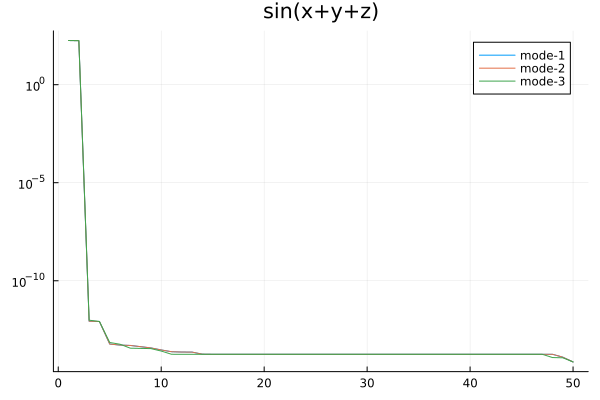
\includegraphics[width=0.85\textwidth]{../figures/p1.png}
\end{figure}

\vspace{1.5em}

\textbf{2}. $ 1/\sqrt{x^2+y^2+z^2+\epsilon^2} $

\vspace{1em}

The ranks are (14, 14, 14) which is balanced but it contains higher rank. This function is radially symmetric which means the function depends only on the distance from the origin.

\begin{figure}[H]
    \centering
    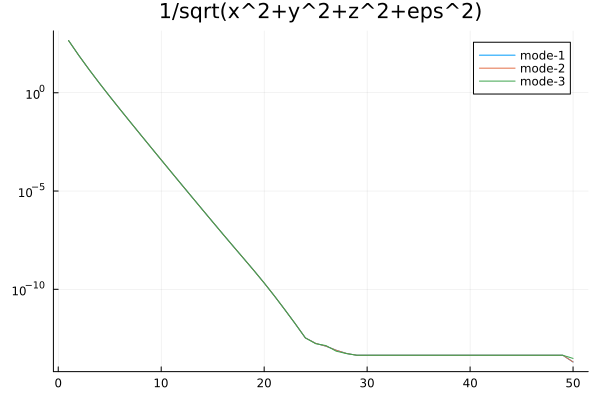
\includegraphics[width=0.85\textwidth]{../figures/p2.png}
\end{figure}

\vspace{1.5em}

\textbf{3}. $ tanh(10(x^2+y^2-z))$

\vspace{1em}

The ranks are (24, 24, 29) which is unbalanced. This function treats the variables asymmetrically. $x,y$ shows quadratically and symmetrically but $z$ appears linearly and contains opposite sign. 

\begin{figure}[H]
    \centering
    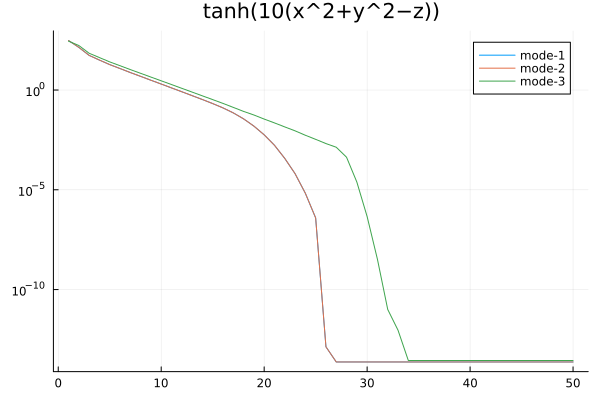
\includegraphics[width=0.85\textwidth]{../figures/p3.png}
\end{figure}

\vspace{1em}

Let
\[
A = G \times _1 U ^{(1)} \times _2 U ^{(2)} \times _3 U ^{(3)}
\]
and
\[
B = H\times _1 W ^{(1)} \times _2 W ^{(2)} \times _3 W ^{(3)}
\]
$G, H$ are core tensor and $U^{(n)}, W^{(n)}$ are factor matrices and $\times_n$ is mode-n product. Frobenius of those two tensors is 
\[
(A,B)_F = \sum_{i_1,i_2,i_3} A_{i_1,i_2,i_3} B_{i_1,i_2,i_3}
\]
when we apply tucker structure, since
\[
A_{i_1,i_2,i_3} = \sum_{j_1,j_2,j_3} G _{j_1,j_2,j_3} U ^{(1)}_{i_1,j_1} U ^{(2)} _{1_2,j_2}  U ^{(3)}_{i_3,j_3}
\]
\[
B_{i_1,i_2,i_3} = \sum_{k_1,k_2,k_3} H _{k_1,k_2,k_3} W ^{(1)}_{i_1,k_1} W ^{(2)} _{1_2,k_2}  W ^{(3)}_{i_3,k_3}
\]
the frobenius formula definition is equal to 
\[
(A,B)_F=\sum_{j_1,j_2,j_3}\sum_{k_1,k_2,k_3} G _{j_1,j_2,j_3} H _{k_1,k_2,k_3} \left( U^{(1)} \right)^T W^{(1)}_{j_1,k_1} \left( U^{(2)} \right)^T W^{(2)}_{j_2,k_2} \left( U^{(3)} \right)^T W^{(3)}_{j_3,k_3}
\]
that is the final inner formula based on multiplication of each core tensors and factor matrices of each mode. This is effective since its computational cost is lower than dense tensor which indicates that the computational speed is faster than normal.

\subsection{Show the tucker structure of A + B}

With ranks $r_1^A, r_2^A, r_3^A$ and $r_1^B, r_2^B, r_3^B$, the sume is all basis vectors from A and B. Therefore, the factor matrices for the sum should have all columns from both tensors.
\[
U^{sum,(n)} = [U^{A,(n)} U^{B, (n)}]
\]
which is equal to
\[
r_1^A + r_1^B, r_2^A +r_2^B, r_3^A+r_3^B 
\]
that is the new multilinear rank.

\vspace{1em}

The new core tensor of A+B is $U^{(n)} = [U^{A,(n)} U^{B, (n)}]$ and core tensor $G_A , G_B$ each that is a block-diagonal tensor.
\[
G_{sum}=\begin{bmatrix}
G_A&0\\0&G_B
\end{bmatrix}
\]
since $G_A$ multiplies the column of $U^A$ and $G_B$ multiplies the column of $U^B$ in separate blocks.

\vspace{1.5em}

\subsection{Implement tucker functions}

\textbf{tucker\_add function}

\begin{lstlisting}
function tucker_add(A::Tucker3, B::Tucker3)::Tucker3
    U1_new = hcat(A.U1, B.U1)   
    U2_new = hcat(A.U2, B.U2)
    U3_new = hcat(A.U3, B.U3)  

    r1A, r2A, r3A = size(A.G)
    r1B, r2B, r3B = size(B.G)

    G_new = zeros(r1A+r1B, r2A+r2B, r3A+r3B)
    G_new[1:r1A, 1:r2A, 1:r3A] = A.G
    G_new[r1A+1:end, r2A+1:end, r3A+1:end] = B.G

    return Tucker3(G_new, U1_new, U2_new, U3_new)
end
\end{lstlisting}

This function adds tucker A and B that use its own basis vectors. A+B concatenate columns and the cores do not mix and it does contain block-diagnoal core.

\textbf{tucker\_sum function}

\begin{lstlisting}
function tucker_sum(terms::Vector{Tucker3}, tol::Float64)::Tucker3
    result = tucker_round(terms[1], tol)
    for i in 2:length(terms)
        result = tucker_round(tucker_add(result, terms[i]), tol)
    end
    return result
end
\end{lstlisting}

This function sums a
vector of Tucker tensors and recompresses the result with tucker\_round.


\textbf{Verification}

\begin{lstlisting}
include("../src/unfold.jl")
include("../src/mode.product.jl")
include("../src/tucker3.jl")
include("../src/tucker_3.jl")
include("../src/todense.jl")
include("../src/tucker_inner.jl")
include("../src/tucker_add.jl")
include("../src/tucker_sum.jl")

using Test
using LinearAlgebra

@testset "tucker_sum test" begin
    U1 = Matrix(I, 10, 10)[:, 1:2]
    U2 = Matrix(I, 10, 10)[:, 1:2]
    U3 = Matrix(I, 10, 10)[:, 1:2]

    Ga = ones(2,2,2)           
    Gb = reshape(1:8, 2,2,2)      

    A = Tucker3(Ga, U1, U2, U3)
    B = Tucker3(Gb, U1, U2, U3)

    dense_exact = todense(A) + todense(B)

    Tsum = tucker_sum([A, B], 1e-12)
    dense_tucker = todense(Tsum)

    err = norm(dense_tucker - dense_exact) / norm(dense_exact)

    @test err < 1e-10
end
\end{lstlisting}

This test contains factor matrices and cores. We get its true sum of dense tensors and it does match with the tucker sum function with error that is less than 1e-10.
It verifies tucker sum function works perfectly.

\textbf{applyL\_tucker function}

\begin{lstlisting}
include("tucker_sum.jl")

function applyL_tucker(W::Tucker3, Dx, Dy, Dz, tol)
    G  = W.G
    U1 = W.U1
    U2 = W.U2
    U3 = W.U3

    T1 = Tucker3(G, Dx * U1, U2, U3)
    T2 = Tucker3(G, U1, Dy * U2, U3)
    T3 = Tucker3(G, U1, U2, Dz * U3)

    return tucker_sum([T1, T2, T3], tol)
end

\end{lstlisting}
It uses tucker sum function to keep the rank under control and it uses the tucker structure directly.

\textbf{step\_and\_truncate solver}

\begin{lstlisting}
include("../src/unfold.jl")
include("../src/mode.product.jl")
include("../src/tucker3.jl")
include("../src/tucker_3.jl")
include("../src/todense.jl")
include("../src/tucker_inner.jl")
include("../src/tucker_add.jl")
include("../src/tucker_sum.jl")
include("../src/applyL_tucker.jl")
using LinearAlgebra
# 7-3 step and truncate 
n = 32
h = 2 * pi/n
x = range(0, 2*pi - h, length=n)
function D_spectral(n)
    h = 2*pi / n
    x = range(0, 2*pi - h, length=n)
    D = zeros(n, n)
    for i in 1:n, j in 1:n
        if i != j
            D[i,j] = 0.5 * (-1)^(i-j) * cot((i-j)*pi/n)
        end
    end
    return D * (2*pi / (n*h))
end
Dx = D_spectral(n)
Dy = D_spectral(n)
Dz = D_spectral(n)

function taylor_step_tucker(W, Dx, Dy, Dz, dt, p, tol)
    terms = [tucker_round(W, tol)]
    Wk = tucker_round(W, tol)
    for k in 1:p
        Wk = applyL_tucker(Wk, Dx, Dy, Dz, tol)
        scale = dt^k / factorial(k)
        push!(terms, Tucker3(Wk.G * scale, Wk.U1, Wk.U2, Wk.U3))
    end
    return tucker_sum(terms, tol)
end

function run_step_and_truncate()
    u0_dense = [sin(xi)*sin(yj)*sin(zk)
                for xi in x, yj in x, zk in x]

    dt = 0.1
    p = 4
    T = 2*pi
    N_steps = round(Int, T/dt)
    tol = dt^(p+1)

    W = Tucker3(u0_dense, tol)
    rank_history = Tuple{Int,Int,Int}[]
    t0 = time()

    for step in 1:N_steps
        W = taylor_step_tucker(W, Dx, Dy, Dz, dt, p, tol)
        push!(rank_history, (size(W.U1,2), size(W.U2,2), size(W.U3,2)))
        if step % 10 == 0
            elapsed = round(time()-t0, digits=1)
            println("step=$step/$(N_steps), ranks=$(rank_history[end]), t=$(elapsed)s")
        end
    end

    println("Finished $N_steps steps")
    for (step, ranks) in enumerate(rank_history)
        println("step=$step ranks=$ranks")
    end

    return rank_history
end

run_step_and_truncate()
\end{lstlisting}

For the 3D advection equation, I implemented the step and truncate time stepping method in tukcer format with the taylor method of order p = 4. Tolerance was chosen as $10^{-5}$ as required. The solver is extremely slow since the taylor method repeatedly applies the operator to the current tucker tensor. This is fundamentally much more expensive than RK4 step and truncate from Lab 1, which only requires four operator evaluations per step.

\subsection{Show each term of $W$ is Tucker}

We are given that
\[
\mathcal{L}(W) = D_x \times_1 W + D_y \times_2 W + D_z \times_3 W
\]
and let
\[
W = G \times_1 U_1 \times_2 U_2 \times_3 U_3
\]
then
\[
D_x \times_1 W = D_x \times_1 G \times_1 U_1 \times_2 U_2 \times_3 U_3
\]
as mode-1 product with $D_x$, it also associates.
\[
D_x \times_1 W = G \times_1  D_x U_1 \times_2 U_2 \times_3 U_3
\]
which contains same core G and factor matrices-tucker structure. Since $D_x U_1$ has rank of $n\times r_1$ which is the rank at most $r_1$-their rank stays same.
When we apply it for every terms,
\[
D_y \times_2 W = G \times_1  U_1 \times_2 D_y U_2 \times_3 U_3
\]
\[
D_z \times_3 W = G \times_1  U_1 \times_2 U_2 \times_3 D_z U_3
\]
this is a tucker tensor with rank at most $r_1, r_2, r_3$ since they have same number of columns as the original factor matrices.

\subsection{Computing Errors}

\begin{lstlisting}
include("../src/unfold.jl")
include("../src/mode.product.jl")
include("../src/tucker3.jl")
include("../src/tucker_3.jl")
include("../src/todense.jl")
include("../src/tucker_inner.jl")
include("../src/tucker_add.jl")
include("../src/tucker_sum.jl")
include("../src/applyL_tucker.jl")
using LinearAlgebra
using Printf

function D_spectral(n)
    h = 2*pi / n
    D = zeros(n, n)
    for i in 1:n, j in 1:n
        if i != j
            D[i,j] = 0.5 * (-1)^(i-j) * cot((i-j)*pi/n)
        end
    end
    return D * (2*pi / (n*h))
end

function taylor_step_tucker(W, Dx, Dy, Dz, dt, p, tol)
    terms = [tucker_round(W, tol)]
    Wk = tucker_round(W, tol)
    for k in 1:p
        Wk = applyL_tucker(Wk, Dx, Dy, Dz, tol)
        scale = dt^k / factorial(k)
        push!(terms, Tucker3(Wk.G * scale, Wk.U1, Wk.U2, Wk.U3))
    end
    return tucker_sum(terms, tol)
end

n = 32  
h = 2*pi / n
x = range(0, 2*pi - h, length=n)
Dx = D_spectral(n)
Dy = D_spectral(n)
Dz = D_spectral(n)

u0_dense = [sin(xi)*sin(yj)*sin(zk) for xi in x, yj in x, zk in x]
u_ref = copy(u0_dense)  # exact solution at T=2*pi equals u0

p = 4
prev_ratio = nothing

println("Convergence test (n=$n, p=$p)")
println("="^55)
println("dt       | error        | dt^p        | ratio")
println("-"^55)

for dt in [0.2, 0.1, 0.05]
    tol = dt^(p+1)
    N_steps = round(Int, 2*pi/dt)

    W = Tucker3(u0_dense, tol)
    t0 = time()

    for step in 1:N_steps
        W = taylor_step_tucker(W, Dx, Dy, Dz, dt, p, tol)
    end

    err = h^(3/2) * norm(todense(W) - u_ref)
    ratio = err / dt^p
    elapsed = round(time()-t0, digits=1)

    @printf("dt=%.3f | err=%.4e | dt^p=%.4e | ratio=%.4f  (%.1fs)\n",
            dt, err, dt^p, ratio, elapsed)

    global prev_ratio = ratio
end
\end{lstlisting}

The convergence test uses a 4th order taylor step-and-truncate method. Each steps produces three tucker tensors and each taylor term adds another tensor to the sum. This indicates that the ranks grow gradually and each truncation requires an SVD of the tucker core. In conclusion, this method is computationally expensive. Since I verified the temporal convergence rate, this method successfully implements 4th order.


\end{document}